\documentclass[]{article}
\usepackage{lmodern}
\usepackage{amssymb,amsmath}
\usepackage{ifxetex,ifluatex}
\usepackage{fixltx2e} % provides \textsubscript
\ifnum 0\ifxetex 1\fi\ifluatex 1\fi=0 % if pdftex
  \usepackage[T1]{fontenc}
  \usepackage[utf8]{inputenc}
\else % if luatex or xelatex
  \ifxetex
    \usepackage{mathspec}
  \else
    \usepackage{fontspec}
  \fi
  \defaultfontfeatures{Ligatures=TeX,Scale=MatchLowercase}
\fi
% use upquote if available, for straight quotes in verbatim environments
\IfFileExists{upquote.sty}{\usepackage{upquote}}{}
% use microtype if available
\IfFileExists{microtype.sty}{%
\usepackage{microtype}
\UseMicrotypeSet[protrusion]{basicmath} % disable protrusion for tt fonts
}{}
\usepackage[margin=1in]{geometry}
\usepackage{hyperref}
\PassOptionsToPackage{usenames,dvipsnames}{color} % color is loaded by hyperref
\hypersetup{unicode=true,
            pdftitle={CoronaNet COVID-19 Government Response Event Dataset},
            pdfauthor={Cindy Cheng1,; Joan Barceló2; Allison Spencer Hartnett3; Robert Kubinec2; Luca Messerschmidt1},
            colorlinks=true,
            linkcolor=Maroon,
            citecolor=Blue,
            urlcolor=blue,
            breaklinks=true}
\urlstyle{same}  % don't use monospace font for urls
\usepackage{longtable,booktabs}
\usepackage{graphicx,grffile}
\makeatletter
\def\maxwidth{\ifdim\Gin@nat@width>\linewidth\linewidth\else\Gin@nat@width\fi}
\def\maxheight{\ifdim\Gin@nat@height>\textheight\textheight\else\Gin@nat@height\fi}
\makeatother
% Scale images if necessary, so that they will not overflow the page
% margins by default, and it is still possible to overwrite the defaults
% using explicit options in \includegraphics[width, height, ...]{}
\setkeys{Gin}{width=\maxwidth,height=\maxheight,keepaspectratio}
\IfFileExists{parskip.sty}{%
\usepackage{parskip}
}{% else
\setlength{\parindent}{0pt}
\setlength{\parskip}{6pt plus 2pt minus 1pt}
}
\setlength{\emergencystretch}{3em}  % prevent overfull lines
\providecommand{\tightlist}{%
  \setlength{\itemsep}{0pt}\setlength{\parskip}{0pt}}
\setcounter{secnumdepth}{5}
% Redefines (sub)paragraphs to behave more like sections
\ifx\paragraph\undefined\else
\let\oldparagraph\paragraph
\renewcommand{\paragraph}[1]{\oldparagraph{#1}\mbox{}}
\fi
\ifx\subparagraph\undefined\else
\let\oldsubparagraph\subparagraph
\renewcommand{\subparagraph}[1]{\oldsubparagraph{#1}\mbox{}}
\fi

%%% Use protect on footnotes to avoid problems with footnotes in titles
\let\rmarkdownfootnote\footnote%
\def\footnote{\protect\rmarkdownfootnote}

%%% Change title format to be more compact
\usepackage{titling}

% Create subtitle command for use in maketitle
\providecommand{\subtitle}[1]{
  \posttitle{
    \begin{center}\large#1\end{center}
    }
}

\setlength{\droptitle}{-2em}

  \title{CoronaNet COVID-19 Government Response Event Dataset}
    \pretitle{\vspace{\droptitle}\centering\huge}
  \posttitle{\par}
    \author{Cindy Cheng\textsuperscript{1,*} \\ Joan Barceló\textsuperscript{2} \\ Allison Spencer Hartnett\textsuperscript{3} \\ Robert Kubinec\textsuperscript{2} \\ Luca Messerschmidt\textsuperscript{1}}
    \preauthor{\centering\large\emph}
  \postauthor{\par}
      \predate{\centering\large\emph}
  \postdate{\par}
    \date{May 16th, 2020}

\linespread{1.6}
\usepackage{booktabs}
\usepackage{longtable}
\usepackage{array}
\usepackage{multirow}
\usepackage{wrapfig}
\usepackage{float}
\usepackage{colortbl}
\usepackage{pdflscape}
\usepackage{tabu}
\usepackage{threeparttable}
\usepackage{threeparttablex}
\usepackage[normalem]{ulem}
\usepackage{makecell}
\usepackage{xcolor}

\usepackage{lineno}
\linenumbers

\begin{document}
\maketitle

\textsuperscript{1} Hochschule für Politik at the Technical University of Munich (TUM) and the TUM School of Governance, Munich, Germany\\
\textsuperscript{2} Social Science Division, New York University Abu Dhabi, Abu Dhabi, United Arab Emirates\\
\textsuperscript{3} Department of Political Science, Yale University, New Haven, United States

\textsuperscript{*} Correspondence: \href{mailto:cindy.cheng@hfp.tum.de}{Cindy Cheng \textless{}\href{mailto:cindy.cheng@hfp.tum.de}{\nolinkurl{cindy.cheng@hfp.tum.de}}\textgreater{}}

\newpage

\hypertarget{abstract}{%
\section*{Abstract}\label{abstract}}
\addcontentsline{toc}{section}{Abstract}

Governments worldwide have implemented countless policies in response to the COVID-19 pandemic. We present an initial public release of a large hand-coded dataset of over 12,000 such policy announcements across more than 190 countries. The dataset is updated daily, with a 5-day lag for validity checking. We document policies across numerous dimensions, including the type of policy; national vs.~sub-national enforcement; the specific human group and geographic region targeted by the policy; and the time frame within which each policy is implemented. We further analyze the dataset using a Bayesian measurement model which shows the quick acceleration of the adoption of costly policies across countries beginning in mid-March and continuing to the present. We believe that the data will be instrumental for helping policy makers and researchers assess, among other objectives, how effective different policies are in addressing the spread and health outcomes of COVID-19.

\hypertarget{introduction}{%
\section*{Introduction}\label{introduction}}
\addcontentsline{toc}{section}{Introduction}

Governments all around the world have implemented an astonishing number and variety of policies in reaction to the COVID-19 pandemic in a very short time frame. However, policy makers and researchers have to date lacked access to the quality, up-to-date data they need for conducting rigorous analyses of whether, how, and to what degree these fast changing policies have worked in brunting the health, political and economic effects of the pandemic. To address this concern, in this paper, we present the CoronaNet COVID-19 Government Response Event Dataset, which provides fine-grained, monadic and dyadic data on policy actions taken by governments across the world since the Chinese government first reported the COVID-19 outbreak on December 31, 2019. At the time of writing, the dataset covers the policy actions of 196 countries up until 2020-05-08, for a total of 12601 events.

With the help of a team of over 260 research assistants in 18 time zones, we are releasing the data on a daily basis. We are implementing a five-day lag between data collection and release to evaluate and validate ongoing coding efforts for random samples of the data to ensure the best possible quality given the considerable time constraints. More specifically, the CoronaNet dataset collects daily data on government policy actions taken in response to COVID-19 across the following dimensions:

\begin{itemize}
\tightlist
\item
  The type of government policy implemented (e.g.~quarantine, closure of schools {[}16 total{]})
\item
  The level of government initiating the action (e.g.~national, provincial)
\item
  The geographical target of the policy action, if applicable (e.g.~national, provincial, municipal)
\item
  The human or material target of the policy action, if applicable (e.g.~travelers, masks)
\item
  The directionality of the policy action, if applicable (e.g.~inbound, outbound, both)
\item
  The mechanism of travel that the policy action targets, if applicable (e.g.~flights, trains)
\item
  The enforcement with the policy action (e.g.~mandatory, voluntary)
\item
  The enforcer of the policy action (e.g.~national government, military)
\item
  The timing of the policy action (e.g.~date announced, date implemented)
\end{itemize}

Though government responses to the COVID-19 pandemic have inaugurated unprecedented changes in how billions of people live their lives, they draw on the lessons learned from the endless series of pandemics and epidemics that came before. Indeed, the earliest written sources document how ancient Mesopotamians responded to the constant threat of epidemic by, on the one hand drawing on spiritual practices and on the other hand, isolating people showing the first symptoms of a disease from others.\textsuperscript{1,2} As time has marched forward, pandemics and epidemics have consistently and dramatically changed the course of human history\textsuperscript{3--7} and governments have continued to implement a variety of policies in response.\textsuperscript{1,8,9} Throughout it all, the collection of reliable data has helped advance collective understanding of which policies are effective in curbing the effects of a given disease outbreak.\textsuperscript{10,11} This is no trivial task given that a policy that is effective in one context may be ineffective in another due to a whole host of potentially conditioning factors, including the pathogenesis of the particular disease\textsuperscript{12,13}, the characteristics of the underlying population\textsuperscript{14--17}, and the available medical\textsuperscript{18,19} and communication\textsuperscript{20--23} technology at the time.

We believe that the data presented in this paper can similarly help policy makers and researchers assess how effective different policies are in addressing the spread and health outcomes of COVID-19\textsuperscript{24}. While available research is necessarily preliminary, it suggests that which policies governments have implemented in response to COVID-19\textsuperscript{25--27}, when they decided to implement them\textsuperscript{29,30}, who they were targeted toward\textsuperscript{31,32} and what state capacity they possessed to do so\textsuperscript{33,34} have all significantly influenced how the virus has affected health outcomes both within and across different country contexts\textsuperscript{35,36}, all of which is readily captured by this dataset. Equally important is understanding why countries adopt different policies, with early analyses suggesting that institutional and political factors, e.g.~the authoritarian or democratic nature of a country's institutions\textsuperscript{37} or its level of political partisanship\textsuperscript{38}, play an important role. These findings will not only help improve the global response to the current crisis, but can also build an influential foundation of knowledge for responding to future outbreaks\textsuperscript{39,40}.

Meanwhile, given the exogenous timing of the initial outbreak in Wuhan, China, government policies made in reaction to the COVID-19 pandemic constitute the single largest natural experiment in recent memory, allowing researchers to improve causal inference in any number of fields. Indeed, government reactions to the COVID-19 pandemic may forward our understanding of a wide-range of social phenomena, from the evolution of political institutions\textsuperscript{41--45} to the progression of economic development\textsuperscript{46--50} and the stability of financial markets\textsuperscript{51,52} to say nothing of what we might learn about environmental economics\textsuperscript{53,54}, mental health\textsuperscript{55,56}, disaster response\textsuperscript{57,58} and disaster preparedness\textsuperscript{59--61}. Some initial analyses suggest that the COVID-19 pandemic has already led to authoritarian backsliding in some countries\textsuperscript{62}, unprecedented shocks to economies around the world\textsuperscript{63--66}, and serious negative mental health effects for millions of people\textsuperscript{67,68}. While scholars have always sought to understand how large-scale historical events have shaped contemporary phenomena, modern technological tools allow us to document such events more quickly and more precisely than ever before.

Detailed documentation of such policies is all the more important given that policy choices made by one government often depend on the policy choices of other governments. The structure of the data we present in this paper allows researchers and policy-makers not only to examine monadic policy information---i.e., policies targeted to the same political unit that enacted it---but also directed, dyadic policy information---i.e., policies targeted to a political unit that is different from the unit that enacted it. The dyadic data is not limited to only capturing foreign policy dynamics, such as when country A implements a policy that affects citizens of country B, but can also document dynamics within countries, such as when central governments enact policies targeted to sub-national political entities. Given its dyadic structure, the dataset further enables critical analyses of the links and interdependencies between and within countries, including patterns of policy learning and diffusion across governments, as well as of cooperative and conflictual relationships in global crisis governance.

In what follows, we provide a description of the data, as well as an application of the data in which we model policy activity of countries over time. Using a Bayesian dynamic item-response theory model, we produce a statistically valid index that categorizes countries in terms of their responses to the pandemic, and further shows how quickly policy responses have changed over time. We document clear evidence of rapid policy diffusion of harsh measures in response to the virus, indicating some of the most extensive evidence of this type of diffusion ever documented. In the methodology section, we provide a thorough discussion of the methodology used to create this index, to collate the dataset and to manage the more than 260 research assistants coding this data around the world in real time.

\hypertarget{results}{%
\section*{Results}\label{results}}
\addcontentsline{toc}{section}{Results}

In this section, we first present some descriptive statistics that illustrate how government policy toward COVID-19 has varied across key variables. We then present our new index for tracking how active governments have been with regard to announcing policies targeting COVID-19 across countries and over time.

\hypertarget{descriptive-statistics}{%
\subsection*{Descriptive Statistics}\label{descriptive-statistics}}
\addcontentsline{toc}{subsection}{Descriptive Statistics}

Here we present some descriptive statistics for key variables available in the dataset. In Table 1, for each policy type we present cumulative totals for the number of policies and the number of countries which have implemented that policy, an average value for the number of countries a policy targets, and percentages in terms how stringently a policy is enforced. While, we highlight the number of targeted countries in this table, we note that our data also captures other potential geographic targets not shown in the table. For instance, it is possible for a national policy to be targeted toward one or more sub-national provinces or a provincial policy to be targeted toward one or more sub-provincial regions.

Table 1 shows that the policy most governments have implemented in reaction to COVID-19 is external border restrictions, i.e.~policies that seek to limit entry or exit across different sovereign jurisdictions. We find that 186 countries have made 1064 policy announcements about such restrictions since December 31, 2019. The second policy that most countries, by our count 169, have implemented is `Closure of Schools', of which we document 1583 such policies.

Meanwhile, the policy that has been implemented the most number of times, at0, has been health resources, that is policies which seek to secure the availability of health-related materials (e.g.~masks), infrastructure (e.g.~hospitals) or personnel (e.g.~doctors) to address the pandemic. The next most common policy in terms of the number of times it has been implemented, at 0, are policies which impose restrictions on non-essential businesses.

However, we note that a strict comparison of policy types by this metric is not perfect, given that, for example, there may be a need for more individualized policies regarding external border restrictions (given the number of countries which a government can restrict travel access to) as opposed to closing schools. We also note that we have more possible sub types for documenting health resources in the survey (21 sub types) than restrictions of non-essential businesses (7 sub types). In the next subsection, we provide a more rigorous method of comparing policies while taking their depth into account.

Additionally, our dataset also shows that the majority of countries in the world are a target of an external border restriction, quarantine measure, or health monitoring measure from another country. Moreover, a high percentage of policies documented in our dataset have mandatory enforcement.

In addition, we can look at the cumulative incidence of different types of policies in our data over time, as we show in Figure 1. The figure shows that arguably relatively easy to implement policies like external border restrictions, the forming of task forces, public awareness campaigns, and efforts to increase health resources came relatively early in the course of the pandemic. Relatively more difficult policies to implement like curfews, closures of schools, restrictions of non-essential businesses and restrictions of mass gatherings arrived later.

\begin{figure}
\centering
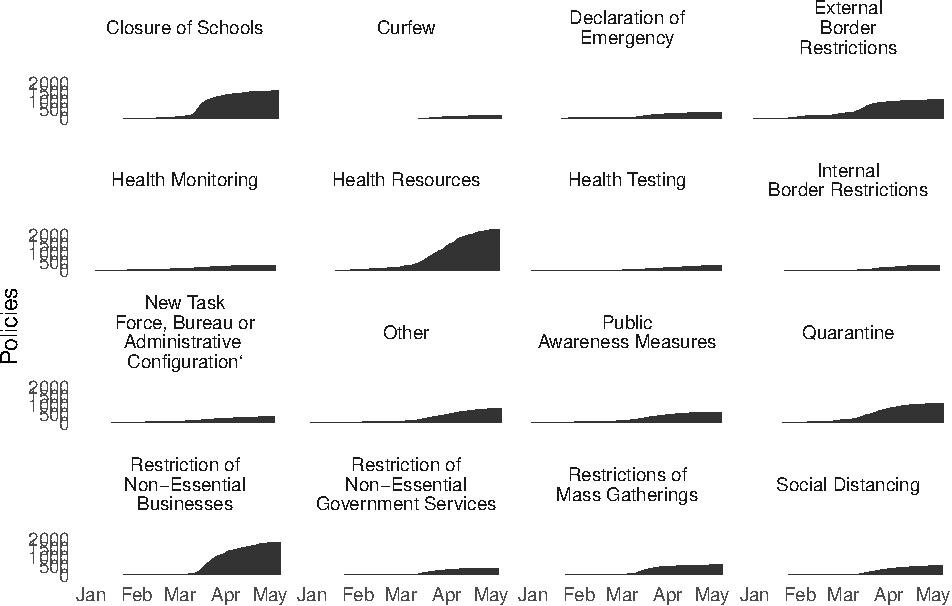
\includegraphics{corona_wp_R1_nature_files/figure-latex/overtime-1.pdf}
\caption{\label{fig:overtime}Cumulative Incidence of Policy Event Types Over Time}
\end{figure}

We can also explore the extent to which other countries are affected by policies that can have a geographic target outside the policy initiator (e.g.~`external border restrictions', `quarantine') across time. For example, in Figure 2, we map a network of bans on inbound flights to European countries initiated by European countries as of March 15, 2020. In the plot, each horizontal line represents a particular country (what in network terminology is called a node). The vertical lines denote whether there was such a flight ban between two countries (what in network terminology is called an edge or a link), and the arrow of the vertical line indicates the direction in which the ban is applied (what in network terminology allows us to capture directed dyads). For instance, in the zoomed in panel inlay in Figure 2, the bottom horizontal line represents Taiwan, and the vertical line connected to it shows that there was a flight ban between Taiwan and Italy. The arrow pointing downwards to Taiwan shows that it was Italy which directed the flight ban against Taiwan. See Longabaugh for more information on how to interpret this plot (2012)\textsuperscript{69}.

Overall, the Figure shows that by March 15, 2020, the governments of Poland and San Marino had banned all flights into Poland and San Marino respectively while the government of Italy banned incoming flights from China, Hong Kong, Macau and Taiwan. Additionally, the governments of Greece and Romania both banned flights from Italy while the government of Albania banned incoming flights from Greece. According to our data, up until this point in time, no other European governments at the national level had banned inbound flights from other countries. The availability of such dyadic data in this dataset may improve inference for any number of analyses which seek to investigate how actions undertaken by different governmental units are linked, including for example on how policies in one country affect health outcomes in another country.

\begin{figure}
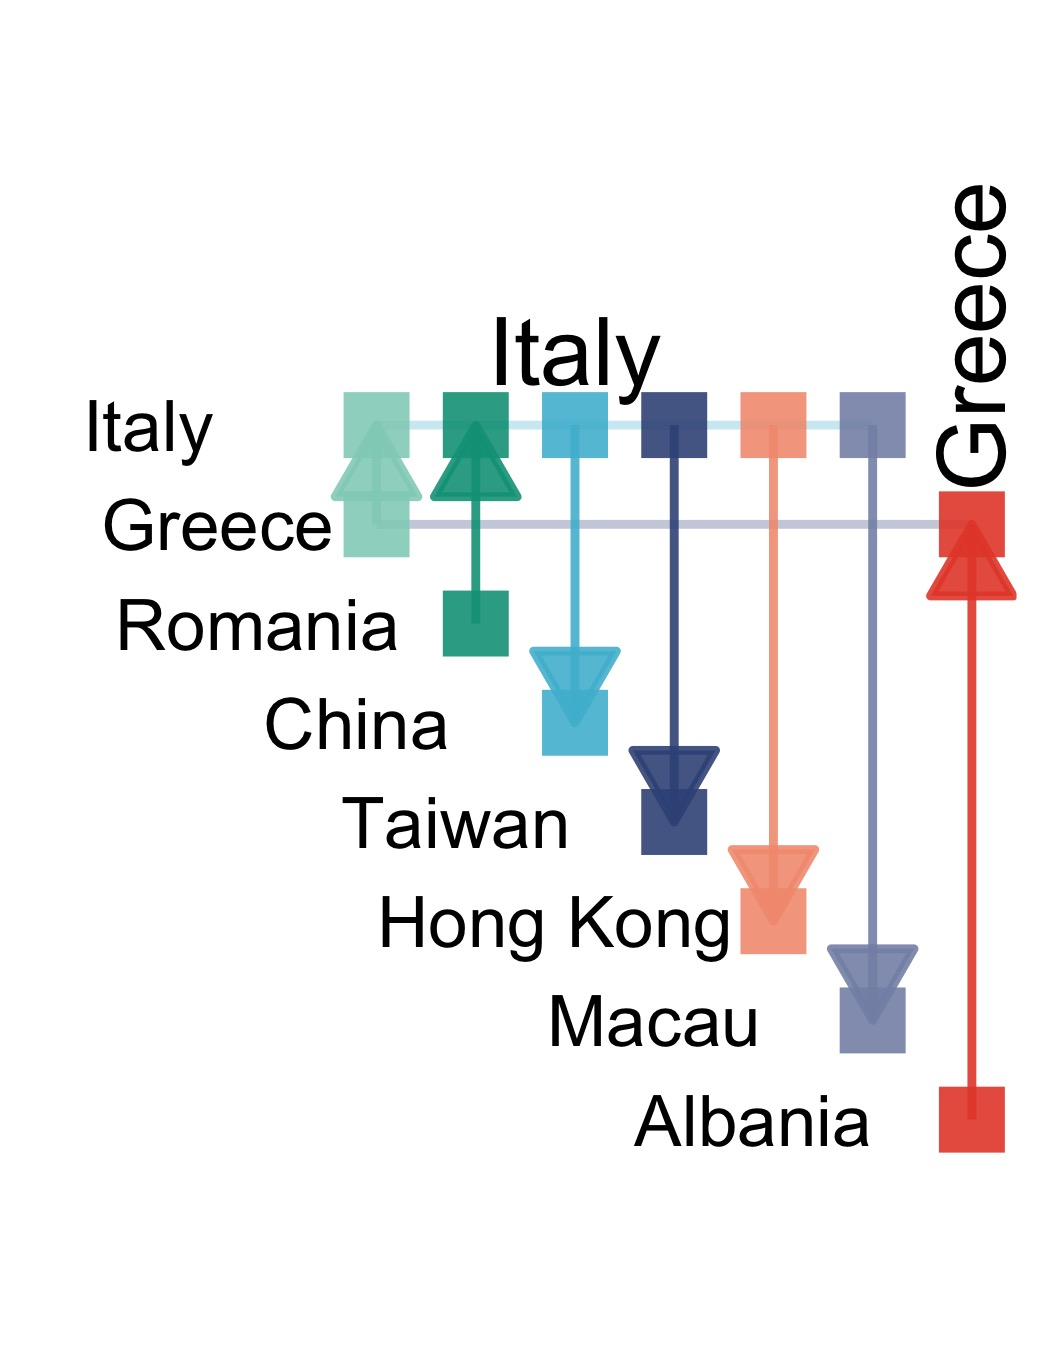
\includegraphics[width=1\linewidth,height=0.5\textheight]{Figure2} \caption{Network Map of Bans on Inbound Flights by European Countries as of March 15, 2020}\label{fig:biofe}
\end{figure}

\hypertarget{government-policy-activity-index}{%
\subsection*{Government Policy Activity Index}\label{government-policy-activity-index}}
\addcontentsline{toc}{subsection}{Government Policy Activity Index}

In this section, we briefly present our new index for tracking the relative government activity with regards to policies targeting COVID-19 across countries and over time. The model is a version of item-response theory known as ideal point modeling which incorporates over-time trends\textsuperscript{70--75}, permitting inference on how a latent construct, in this case total policy activity, responds to changes in the pandemic. To fit the model, the different policy types shown in Table 1, as well as sub-policies within them, were coded in terms of ordinal values, with lower values for sub-national targets of policies and higher values for policies applying to the entire country, or in the case of external border restrictions, to one or more external countries. For instance, internal country policies can take on three possible values: no policy, sub-national policy, or policy covering the whole country. Meanwhile external border restrictions can take on four possible values: no policy, policy targeting one other country, policy targeting multiple countries, and policy targeting all countries in the world (i.e., border closure).

We employed ideal point modeling because it can be given a latent utility interpretation\textsuperscript{71}. We assume that each country has an unobserved ``ideal point'' on a uni-dimensional space representing its willingness to impose policies, while each policy likewise has a position on the same space. The relative cost of different policies can be thought of as the distance between a country's ideal point and the ideal point of the policy relative to other policies. While the meaning of this implied cost will vary from country to country, it is likely a combination of the social, political and economic costs of implementing the policy at a given time point.

As countries become more willing to pay the implied cost (i.e.~the latent distance between country and policy decreases), the country's ideal points/policy activity score will rise and they will implement more policies. This interpretation is similar to the traditional item-response theory approach for analyzing test questions in which students who correctly answer more questions on a test are considered to have higher ``ability''\textsuperscript{76,77}. Following this logic, we are able to estimate latent country scores that represent the readiness of a country to impose a set number of policies. The implied cost of policies is estimated via discrimination parameters, which indicate how strongly policies discriminate between countries.

The country-level policy activity score is further allowed to vary over time in a random-walk process with a country-specific variance parameter to incorporate heteroskedasticity\textsuperscript{73}. Incorporating over-time trends explicitly is very important for capturing the nuances of policy implementation over time. For example, countries that impose more restrictive policies at an earlier date will be rewarded with higher policy activity scores compared to those who impose such policies at a later date. Imposing a given policy when most countries have already imposed them will result in little if any change in the policy activity score.

The advantage of employing a statistical model, rather than simply summing across policies, is that the index ends up as a weighted average, where the weights are derived from the probability that a certain policy is implemented. In other words, while many countries set up task forces, relatively few imposed curfews at an early stage. As a result, the model adjusts for these distinctions, producing a score that aggregates across the patterns in the data.

Furthermore, because the model is stochastic, it is robust to some of the coding errors of the kind that often occur in these types of datasets. As we discuss in our validation section, while we are continuing to validate the data on a daily basis, the massive speed and scope of data collection means that we cannot identify all issues with the data in real time. However, the measurement model employed only requires us to assume that on average the policy codings are correct, not that they are correct for each instance. Coding error, such as incorrectly selecting a policy type, will propagate through the model as higher uncertainty intervals, but will not affect average posterior estimates. As our data quality improves, and we are able to collect more data over time, the model will produce more variegated estimates with smaller uncertainty intervals.

Figure 3 shows the estimated index scores for the 196 countries in our dataset at present, and suggests strong evidence of policy diffusion effects. While information about COVID-19 existed at least as early as January, we do not see large-scale changes occurring in activity scores until March. Furthermore, the trajectories are highly non-linear, with a large number of countries quickly transitioning from relatively low to relatively high scores. This non-linear movement could be due to a variety of factors, including the rapid spread of the virus and policy learning as states observe other states' policy actions. We note that the country that appeared to take the quickest action in the shortest amount of time is New Zealand, as can be seen in Figure 5 where we show over-time variance parameters for each country. For an interactive version of this figure, please see our website.

Of course, a caveat with the index is that we may be missing some possible policy measures that have occurred due to the difficulty in finding them in published sources. However, there is still clear differentiation within the index in terms of when policies were imposed, with some countries starting to impose policies much earlier than others. Furthermore, there is a clear break around March 1st when countries began to impose more stringent policies across the world.

\begin{figure}
\centering
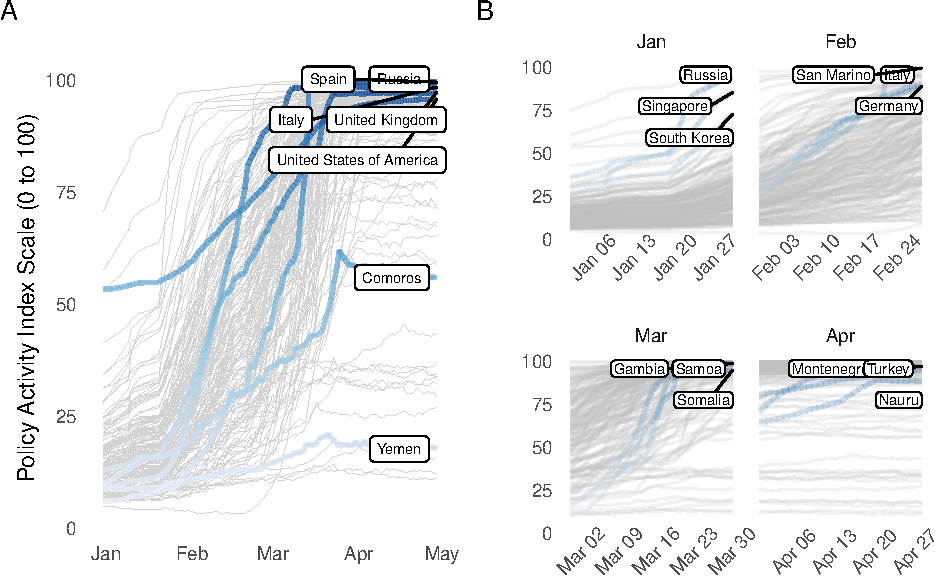
\includegraphics{corona_wp_R1_nature_files/figure-latex/plotindex-1.pdf}
\caption{\label{fig:plotindex}CoronaNet Time-Varying Index of National Policy Activity of Measures Opposing COVID-19 Pandemic. Estimates are derived from Stan, a Markov Chain Monte Carlo sampler. Median posterior estimates are shown. Plot A shows the full distribution of countries, while plot B shows each month separately with the top 3 countries for that month in terms of increases in activity scores from start of the month to the end of the month.}
\end{figure}

Table 2 shows the discrimination parameters from the underlying Bayesian model for each policy type. These parameters suggest which policies governments find relatively difficult or costly to implement, and for that reason tend to separate more active from less active states in terms of response to COVID-19. Two of these policies (Closure of Restaurants and Quarantine at Home) were given fixed values in order to identify the direction and rotation of the latent scale, and so their discrimination parameters are not informative. These policies were chosen as \emph{a priori} we can identify them as being relatively high cost. However, the rest of the parameters were allowed to float, which provides inference as to which policies appear to be the most difficult/costly to implement.

We note that these are average values for the sample. Imposing these policies may be less costly for certain countries or for countries that share certain characteristics, such as having smaller numbers of enrolled students or relatively healthy economies. However, it is important to note that we can see these patterns on a world-wide scale.

At the top of the index we see various business closure policies as the most difficult to implement, while school closures are the next most difficult. Closure of pre-schools, though, as opposed to other school types, appears to be relatively less costly for states to undertake, perhaps because pre-schools do not operate on a full-time basis. Internal border restrictions are considered more difficult to implement than external border restrictions, while relatively straightforward policies like public awareness campaigns, health monitoring and opening new task forces or bureaus are near the bottom of the index. Quarantines placing people in external facilities, such as hotels or government quarantine centers, are also estimated as being less costly than quarantine at home (stay-at-home orders).

Given this distribution of discrimination parameters, we believe the index is a valid representation of the underlying process by which governments progressively impose more difficult policies. As states relax policies, we will further gain information about which policies appear to be more costly as we will be able to factor in the duration for which these policies were implemented. Consistent with our findings, we observe that the announced relaxation policies happening at the time of writing in European countries primarily center on businesses and school openings, suggesting that these policies are uniquely costly to keep in place compared to travel restrictions\textsuperscript{78}.

\hypertarget{methods}{%
\section*{Methods}\label{methods}}
\addcontentsline{toc}{section}{Methods}

In this section, we first provide more detail on the methodology we employed to estimate our government policy action index. We then describe the variables that our dataset provides as well as how they are organized. We then provide detail on the methodology we employed to collect the data.

\hypertarget{time-varying-item-response-model}{%
\subsection*{Time-Varying Item Response Model}\label{time-varying-item-response-model}}
\addcontentsline{toc}{subsection}{Time-Varying Item Response Model}

Our time-varying item response model follows the specification in 79. We review that notation here to show how it relates to classical item-response theory as well as the ideal point modeling literature.

The likelihood function for the model is as follows for a set of countries \(i \in I\), items \(j \in J\), time points \(t \in T\) and ordinal categories \(k \in K\):

\begin{align}
    L(Y_{ijtk}|\alpha_{it},\gamma_j,\beta_j) =  \prod_{i=1}^{I} \prod_{j=1}^{J} \prod_{t=1}^{T}
    \begin{cases} 
    1 -  \zeta(\gamma_j \alpha_{it} - \beta_j - c_1) & \text{if } K = 0 \\
    \zeta(\gamma_j \alpha_i - \beta_j - c_{k-1}) - \zeta(\gamma_j \alpha_{it} - \beta_j - c_{k})       & \text{if } 0 < k < K, \text{ and} \\
    \zeta(\gamma_j \alpha_{it} - \beta_j - c_{k-1}) - 0 & \text{if } k=K
    \end{cases}
\label{eq:basic}
\end{align}

In this equation, the time-varying country parameters \(\alpha_{it}\), also called person abilities or ideal points, are our estimate of policy activity scores. They are estimated jointly with the item (policy type) discrimination parameters \(\gamma_j\) and item difficulty (intercept) parameters \(\beta_j\). To address the ordinal nature of the outcome \(Y_{ijtk}\), ordinal cutpoints \(c_{k}\) are used to model the varying levels of enforcement and geographical targets in the data. The logit function, represented by \(\zeta(\cdot)\), maps the latent scale to probability that a given ordinal outcome is chosen. Because we have two separate type of ordered measures (domestic versus international policies) with either three or four ordered categories, we estimate the model jointly as two ordered logit specifications.

The likelihood in \eqref{eq:basic} is not fully identified due to possible scaling issues with the latent variable \(\alpha_{it}\) (i.e., it has no natural units) and due to potential sign reflection (also called multi-modality) where \(L(Y_{ijtk})\) could be unchanged even if \(\alpha_{it}\) is multiplied by -1. These identification issues are well-known in the literature\textsuperscript{72}, and we resolve them with standard practices. First, we assign a reasonably informative prior distribution on the \(t=1\) ideal points:

\begin{equation}
\alpha_{it=1} \sim N(0,1)
\label{eq:id1}
\end{equation}

We also fix the discrimination parameters \(\gamma_j\) for two items, quarantines and restriction of restaurants and bars, to opposite ends of the latent scale (+1 and -1). Because both of these variables load on the same side of the scale (i.e.~both indicate more policy activity), we reverse the order of the categories for restriction of restaurants and bars. We note that these types of restrictions are not commonly used in traditional IRT, where instead a sign restriction is imposed on all discrimination parameters. We employ the more flexible ideal point specification, which also allows us to test the assumption that all the discrimination parameters load on the same sign (as Table 2 shows, this is true for all of the parameters). The rest of the parameters are given weakly informative prior distributions (note a prior is put over the difference of cutpoints, rather than the cutpoints themselves, to reflect the fact that only the differences between cutpoints have any natural scale):

\begin{align}
\gamma_j &\sim N(0,5)\\
\beta_j &\sim N(0,2)\\
c_k - c_{k-1} &\sim N(0,5)
\label{eq:id2}
\end{align}

Finally, to model the policy scores \(\alpha_{it}\) as a random walk, we assign a prior that is equal to the prior period policy score plus normally-distributed noise:

\begin{align}
\alpha_{it} &\sim N(\alpha_{it-1},\sigma_i)\\
\sigma_i &\sim E(1)
\label{eq:rwc}
\end{align}

The over-time dimension induces a new source of identifiability issues, which we resolve by fixing the variance \(\sigma_i\) of one of the countries (the United States) to 0.1 so that the over-time variance is relative to this constant. This constraint has a similar identification effect to the informative prior on the first period policy activity scores in \eqref{eq:id1}.

\hypertarget{model-convergence}{%
\subsection*{Model Convergence}\label{model-convergence}}
\addcontentsline{toc}{subsection}{Model Convergence}

For estimation, we sample from four Markov Chain Monte Carlo (MCMC) chains with over-dispersed starting values using Stan, a Hamiltonian Markov Chain Monte Carlo (HMC) sampler\textsuperscript{80}. We run the sampler for 800 iterations, 400 of which are discarded as warm-up. While this number of iterations is far less than other MCMC samplers, HMC is far more efficient at exploring the posterior density and we are able to achieve convergence using this number of iterations.

We assess convergence using split-\(\hat{R}\) by fitting four independent chains with over-dispersed starting values. \(\hat{R}\) values for all parameters (which totaled more than 40,000) were 1.01 or less (see plot A in Extended Data Figure 1). Plot B in Figure in Extended Data Figure 1 shows the distribution of effective number of samples for the parameters, which is a way of comparing the auto-correlation in MCMC draws to independent draws without auto-correlation, such as we might obtain from a Monte Carlo simulation. Again, the number of effective samples is quite high, often exceeding the total number of empirical draws. This occurred because Hamiltonian Monte Carlo can produce more informative samples than even a Monte Carlo simulation because it can generate negatively correlated draws that explore the posterior space much more quickly. We also assess convergence using trace plots, one of which is shown below for the time-varying country policy activity scores for the United States. Strong mixing between chains can be observed in the plot. Finally, we report no divergent transitions or iterations where the sampler reached its maximum tree depth, which are both signs of poor mixing in the chains. For these reasons, we are confident than the sampler reached a stationary distribution and was able to adequately explore the high-density regions of the joint posterior.

\begin{figure}
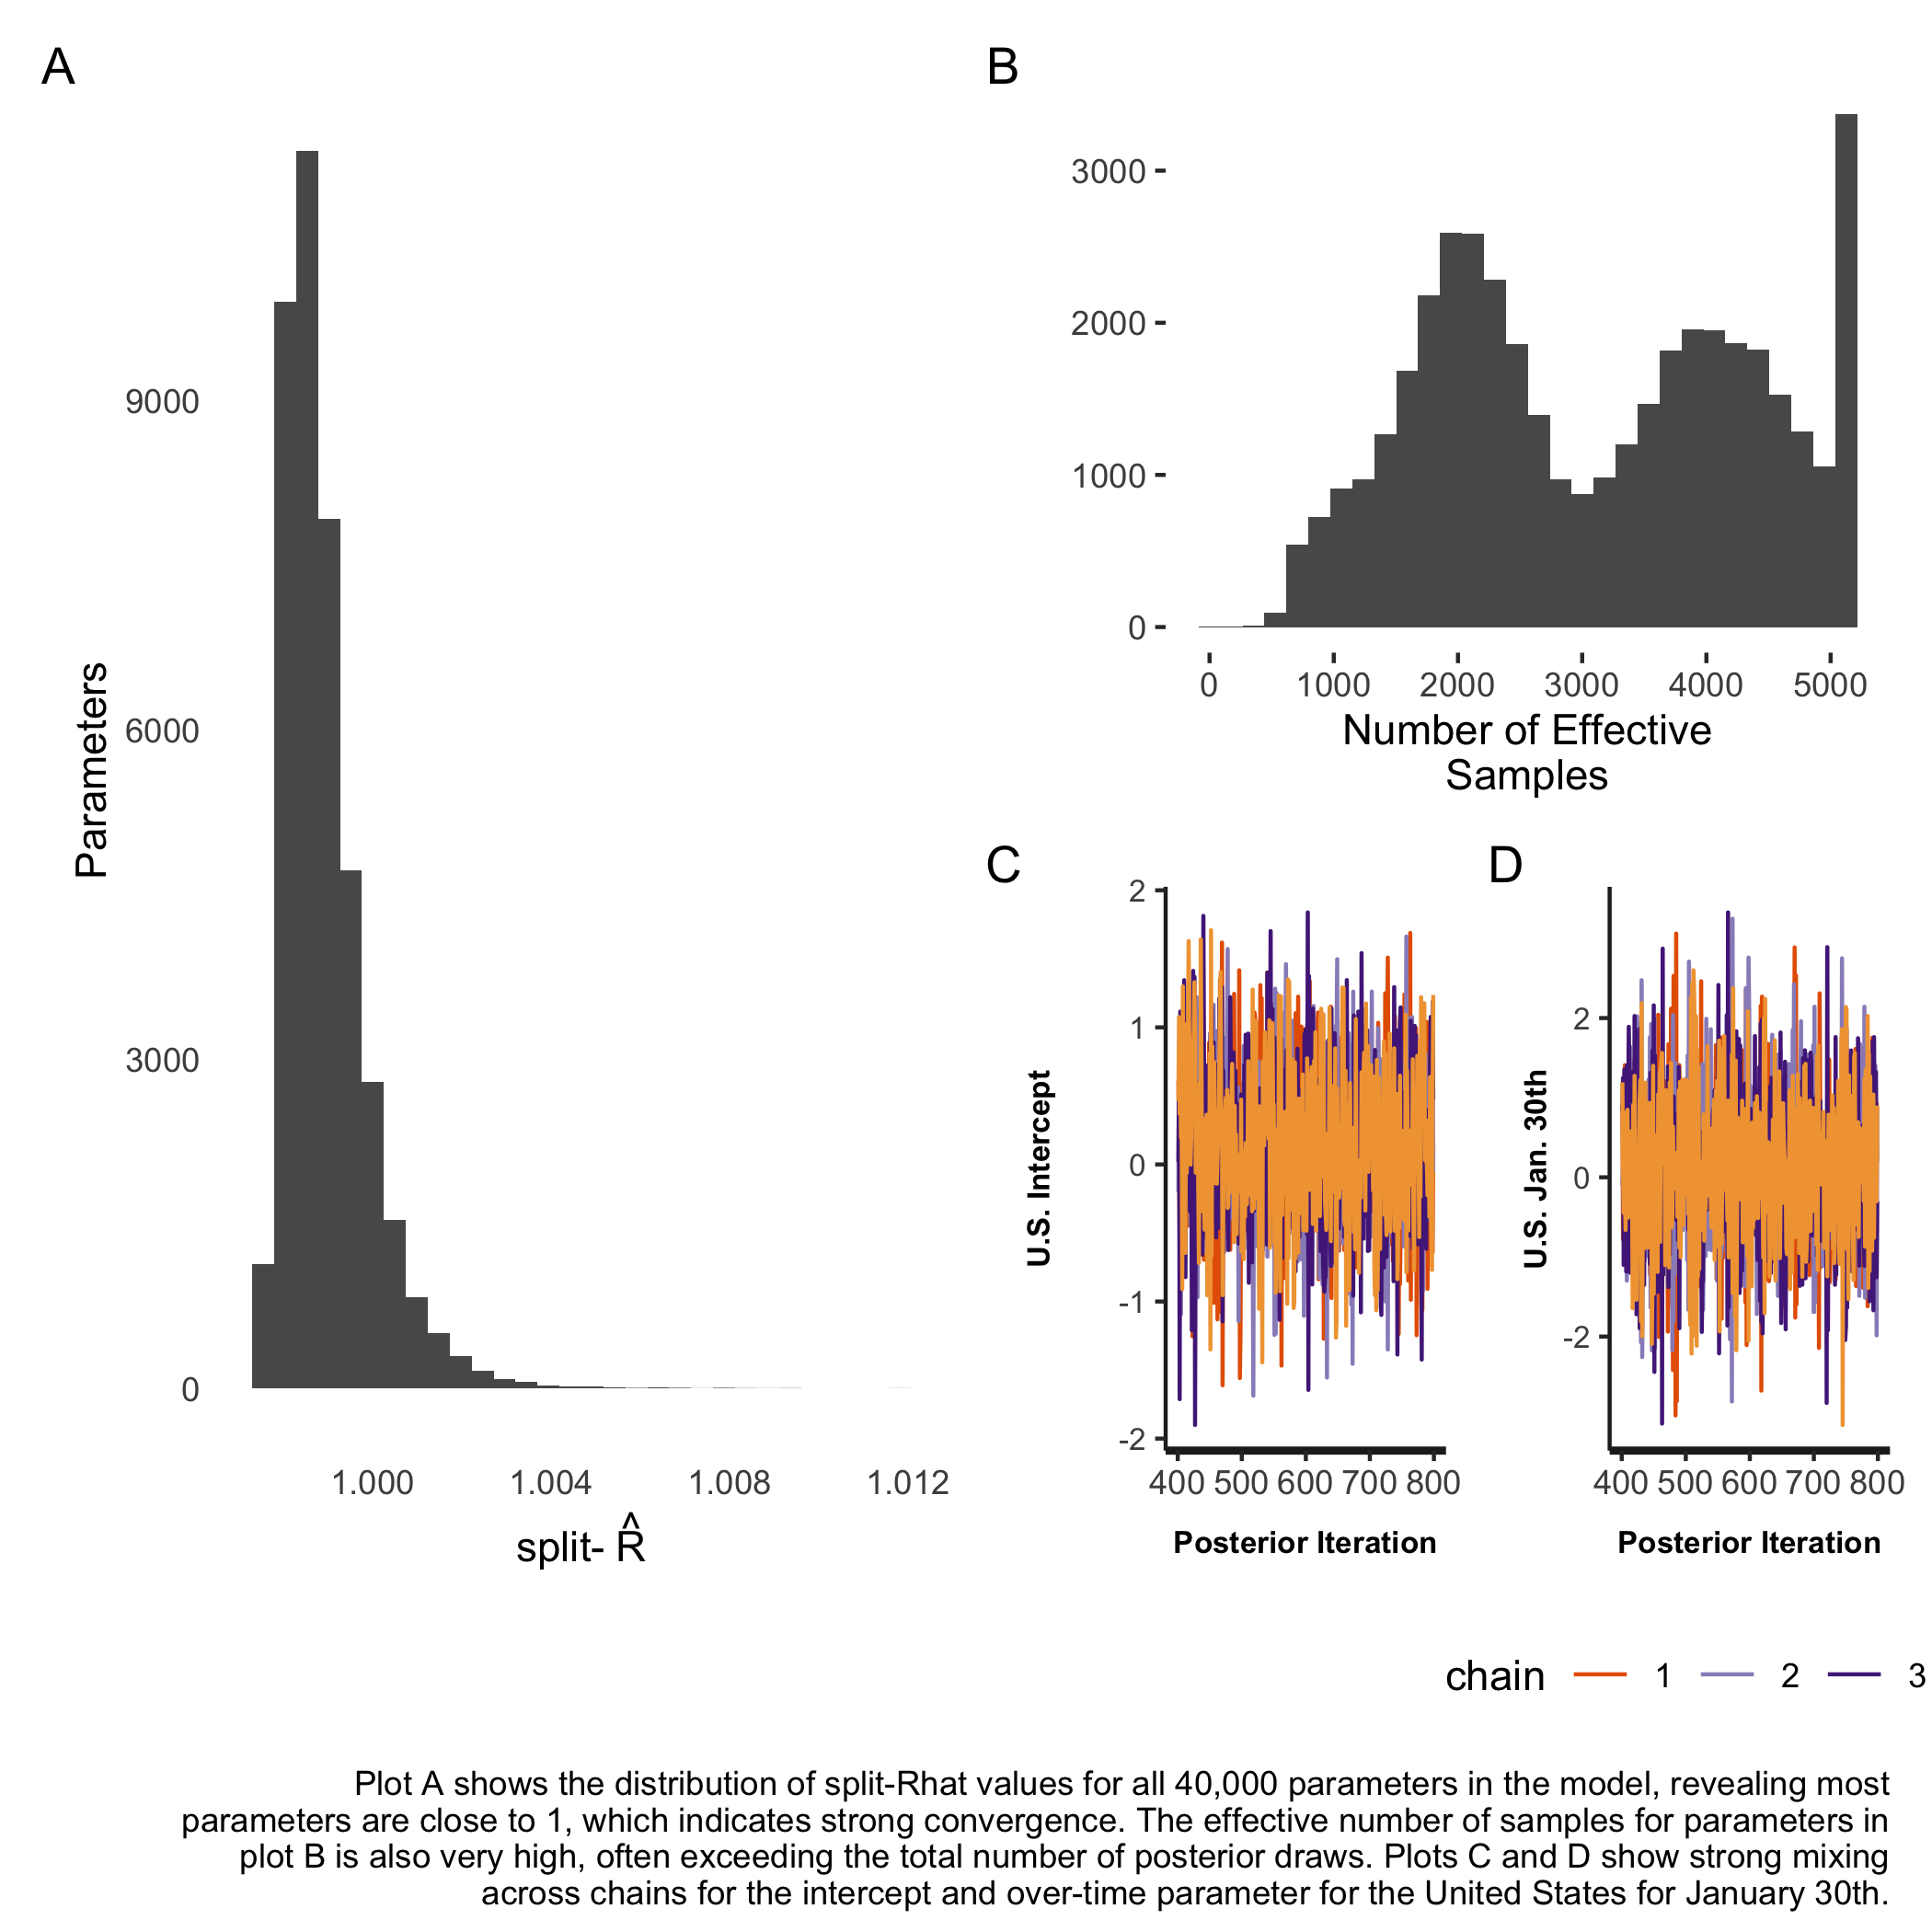
\includegraphics[width=6.46in]{mcmc_evaluate} \caption{Convergence Diagnostics for Random-Walk HMC Fit. Plot A shows the distribution of split-Rhat values for all 40,000 parameters in the model, revealing most parameters are close to 1, which indicates strong convergence. The effective number of samples for parameters in plot B is also very high, often exceeding the total number of posterior draws. Plots C and D show strong mixing across chains for the intercept and over-time parameter for the United States for January 30th.}\label{fig:modelconv}
\end{figure}

\hypertarget{model-validity}{%
\subsection*{Model Validity}\label{model-validity}}
\addcontentsline{toc}{subsection}{Model Validity}

While employing a measurement model ensures robustness to arbitrary data coding errors, it is still necessary to validate the model's over-time process, which imposes some assumptions on how policy activity scores change over time. The use of a random walk implies that policy differences will be relatively stable from one day to the next, which could limit the ability of scores to encompass quick, discontinuous changes\textsuperscript{81}. While we employ this particular specification because it has been applied previously to a variety of empirical phenomena and because of its relative parsimony, we can partially test for whether it captures changes by estimating a static IRT model for each day in the sample. The corresponding estimates represent cross-sections without any time process imposed.

Due to the complexity of comparing the estimates, we plot the results for six countries separately in Figure 4. This figure shows that indeed the cross-sectional estimates can show much more discontinuous jumps, though we note at the same time that there appears to be substantial noise in the estimates as they only incorporate information available at a single day. Nonetheless, while the random-walk estimates certainly exhibit less discontinuous change, they do still allow for very quick divergence in policy activity scores, with France and Russia moving from the bottom to the top of the index in the space of only a few weeks.

\begin{figure}
\centering
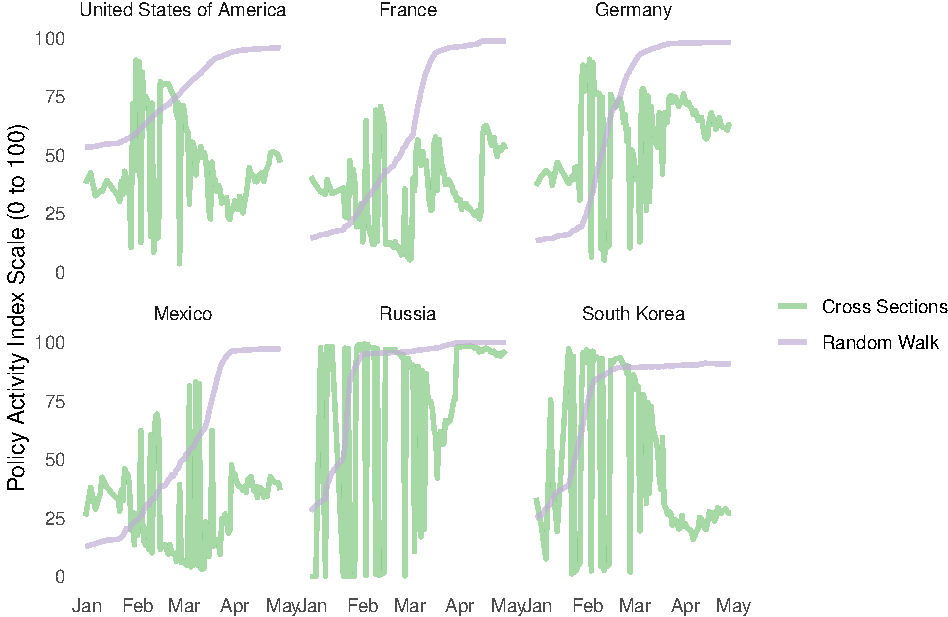
\includegraphics{corona_wp_R1_nature_files/figure-latex/timeest-1.pdf}
\caption{\label{fig:timeest}Comparison of Cross-sectional Estimates of Policy Activity Scores to the Random-Walk Time Series Estimates}
\end{figure}

We note as well that the model is parameterized so that each country has its own variance parameter. This permits the rate of change to vary by country, reducing the concern that the model may be overly restricting change. These variance parameters are shown in Figure 5, sorted in order of increasing over-time variance. These estimates are themselves substantively interesting, as the United States, which was used as the reference category, has actually one of the lowest rates of over-time change, while some countries like New Zealand, Spain and San Marino witnessed the highest variance in policy activity scores. Because, at this time, the index only captures increasing numbers of policies, the variance parameters can be given the interpretation of which countries responded in the shortest period of time across a broad array of policy indicators.

\begin{figure}
\centering
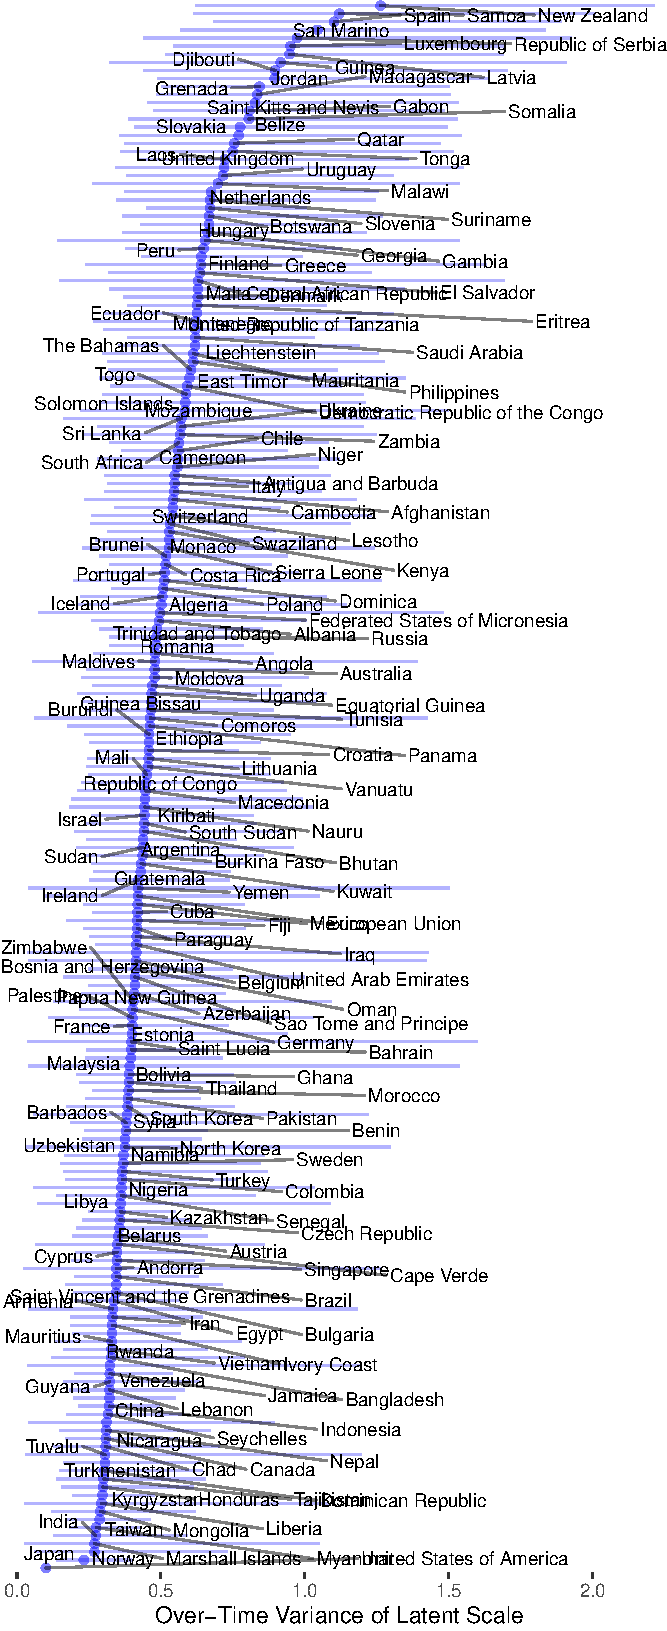
\includegraphics{corona_wp_R1_nature_files/figure-latex/plotvar-1.pdf}
\caption{\label{fig:plotvar}Country-level Variance (Over-time Change) Parameters from Policy Activity Index Estimation}
\end{figure}

\hypertarget{data-schema}{%
\subsection*{Data Schema}\label{data-schema}}
\addcontentsline{toc}{subsection}{Data Schema}

Each unique record documents at the minimum, the following information: the policy type; the name of the country from which a policy originates (if the policy originates from a province or state, that information is also documented. Future versions of the dataset will also include information on whether a policy was initiated from a city or municipality or another level of government); the degree to which a policy must be complied with; the entity enforcing the policy; the date a policy is announced, implemented and ends. Note that sometimes policies are announced without a pre-determined end date. In those cases, this field is left blank.

For all policies, the database further documents information about the geographic target of the policy and the human or material target of a policy. Note however, for some policies, the geographic target may be the same as the policy initiator and in those cases can be considered monadic. Where applicable, we also document the directional flow of the policy, and the mechanism of travel.

All of the information mentioned above is also provided qualitatively via a textual event description. Additional meta-data that is available for all policies include when the record entered into the database and a link for the information source for the policy. See Appendix A in the supplementary materials for a list of currently available fields in the data, along with a list of external data variables such as country-level covariates that are added to daily releases, including COVID-19 tests and cases.

There is a unique record ID for each unique policy announcement per initiating country, which we code at the policy sub type. That is, some policy types are further categorized into sub types. For example, `Quarantine' can be further classified into one or more of the following sub types: `Self-Quarantine', `Government Quarantine', `Quarantine outside the home or government facility', `Quarantine only applies to people of certain ages' and `Other'. Of the 12601 such events in the dataset, we have identified 10798 unique events. That is, some events in the database are updates or changes to existing policies. We link such events over time using a unique ID, which we term the policy ID as opposed to the record ID. An event counts as an update if it deals with a change in either the:

\begin{enumerate}
\def\labelenumi{\arabic{enumi}.}
\tightlist
\item
  The time duration (e.g.~A country lengthens its quarantine to 28 days from 14 days.)
\item
  The quantitative `amount' of the policy (e.g.~A restriction of mass gatherings was previously set at 100 people and now it is set at 50 people).
\item
  A set of other policy dimensions:
\end{enumerate}

\begin{enumerate}
\def\labelenumi{\alph{enumi}.}
\tightlist
\item
  Who the policy applies towards (e.g.~The quarantine used to apply to people of all ages and now it only applies to the elderly).
\item
  The directionality of the policy (e.g.~a travel ban previously banned inbound flights from country X and now bans both inbound and outbound flights to and from country X).
\item
  The travel mechanism (e.g.~a travel ban was previously applied towards all types of travel but now only applies towards flights).
\item
  The compliance rules for the policy (e.g.~The quarantine used to be voluntary but is now mandatory).
\item
  The enforcer of a policy (e.g.~the policy was previously under the purview of the ministry of health but was changed to the ministry of the interior).
\end{enumerate}

A policy counts as a new entry and not an update if it deals with a change in any other dimension, e.g.~the qualitative policy type (e.g.~a quarantine used to mandate a stay in a government facility but now quarantine at home is allowed) or the targeted country (e.g.~quarantine upon arrival was mandated for people traveling from China but now these rules also apply to people traveling from Italy). In those cases, or when a policy is completely cancelled or annulled, the policy is coded as having ended.

\hypertarget{data-collection-methodology}{%
\subsection*{Data Collection Methodology}\label{data-collection-methodology}}
\addcontentsline{toc}{subsection}{Data Collection Methodology}

As researchers learn more about the various health, economic, and social effects of the COVID-19 pandemic, it is crucial that to the greatest extent possible, they have access to data that is reliable, valid, and timely. We have adopted a data collection methodology that we believe optimizes over all three of these constraints.

To collect the data, we recruited more than 260 research assistants (RAs) from colleges and universities around the world, representing 18 out of the 24 time zones. Large social scientific datasets typically rely on experts, coders, or crowd-sourcing to input data. The literature has shown that common coding tasks can be completed via crowd-sourcing\textsuperscript{82,83}, but that there are also limitations to the wisdom of crowds when specific contextual or subject knowledge is required\textsuperscript{84,85}. To address these trade offs, we decided to train current RAs to code our entries, leveraging the benefits of wide-spread recruitment and a diverse pool of country-specific knowledge from across the globe. Data collection started on March 28, 2020 and has proceeded rapidly, reaching 12601 records as of the date of this article. Each RA is responsible for tracking government policy actions for at least one country. RAs were allocated depending on their background, language skills and expressed interest in certain countries\textsuperscript{86}. Note depending on the level of policy coordination at the national level, certain countries were assigned multiple RAs, e.g.~the United States, Germany, or France.

We have also partnered with the machine learning company Jataware to automate the collection of more than 200,000 news articles from around the world related to COVID-19. Jataware employs a natural language processing (NLP) classifier using Bidirectional Encoder Representations from Transformers (BERT) to detect whether a given article is indicative of a governmental policy intervention related to COVID-19. They then apply a secondary NLP classifier to categorize the type of policy intervention based on the definitions in our codebook (e.g.~``declaration of emergency'', ``quarantine'', etc.). Next, Jataware extracts the geospatial and temporal extent of the policy intervention (e.g.~``Washington DC'' and ``March 15, 2020'') whenever possible. The resulting list of news sources is then provided to our RAs as an additional source for manual coding and further data validation.

In what follows, we describe in greater detail how RAs document the policies that they identify using our data collection software instrument, and our post data-collection validation procedure. Please refer to the Appendix B in the supplementary materials for more information on our procedure for on-boarding and training RAs and our system for communicating with and organizing RAs.

\hypertarget{data-collection-software-instrument}{%
\subsubsection*{Data Collection Software Instrument}\label{data-collection-software-instrument}}
\addcontentsline{toc}{subsubsection}{Data Collection Software Instrument}

We designed a Qualtrics survey with survey questions to systematize and streamline the documentation of a given government policy over a wide range of dimensions. With this tool, RAs can easily and efficiently document information about different policy actions by answering the relevant questions posed in the survey (Büthe, Minhas and Lieu, unpublished manuscript). For example, instead of entering the country that initiated a policy action into a spreadsheet, RAs answer the following question in the survey: ``From what country does this policy originate?'' and choose from the available options given in the survey.

By using a survey instrument to collect data, we are able to systematize the collection of very fine-grained data while minimizing coding errors common to tools like shared spreadsheets. The value of this approach of course, depends on the comprehensiveness of the questions posed in the survey, especially in terms of the universe of policy actions that countries have implemented against COVID-19. For example, if the survey only allowed RAs to select `quarantines' as a government policy, it would not capture any data on `external border restrictions', which would seriously reduce the value of the resulting data.

As such, to ensure the comprehensiveness of the data, before designing the survey, we collected in depth, over-time data on policy actions taken by one country since the beginning of the outbreak, Taiwan, as well as cross-national data on travel bans implemented by most countries for a total of 245 events. The specific data source we cross referenced for this effort was the March 20, 2020 version of a New York Times article on travel restrictions across the globe\textsuperscript{87}.

We chose to focus on Taiwan on because of its relative success, as of March 28, 2020, in limiting the negative health consequences of COVID-19 within its borders\textsuperscript{88}. As such, it seemed likely at the time that other countries would choose to emulate some of the policy measures that Taiwan had implemented, which increases the comprehensiveness of the questions we ask in our survey. Indeed at the time of writing, it would appear that some countries have indeed sought to emulate Taiwan's response\textsuperscript{89}.

Meanwhile, by also investigating variation in how different countries around the world have implemented travel restrictions, we have also helped ensure that our survey is able to comprehensively document variation in how an important and commonly used policy tool is applied, e.g., restrictions on different methods of travel (e.g.~flights, cruises), restrictions across borders and within borders, restrictions targeted toward people of different statuses (e.g.~citizens, travelers).

There are many additional benefits of using a survey instrument for data collection, especially in terms of ensuring the reliability and validity of the resulting data:

\begin{enumerate}
\def\labelenumi{\arabic{enumi}.}
\item
  Preventing unforced measurement error: RAs are prevented from entering data into incorrect fields or unknowingly overwriting existing data---as would be possible with manual data entry into a spreadsheet---because RAs can only document one policy action at a time in a given iteration of a survey and do not have access to the full spreadsheet when they are entering in the data.
\item
  Standardizing responses: We are able to ensure that RAs can only choose among standardized responses to the survey questions, which increases the reliability of the data and also reduces the likelihood of measurement error. For example, when RAs choose different dates that we would like them to document (e.g., the date a policy was announced) they are forced to choose from a calendar embedded into the survey which systematizes the day, month and year format that the date is recorded in.
\item
  Minimizing measurement error: A survey instrument allows coding different conditional logics for when certain survey questions are posed. This technique obviates the occurrence of logical fallacies in our data. For example, we are able to avoid situations where an RA might accidentally code the United States as having closed all schools in another country.
\item
  Reduction of missing data: We are able to reduce the amount of missing data in the dataset by using the forced response option in Qualtrics. Where there is truly missing data, there is a text entry at the end of the survey where RAs can describe what difficulties they encountered in collecting information for a particular policy event.
\item
  Reliability of the responses: We increase the reliability of the documentation for each policy by embedding descriptions of different possible responses within the survey. For example, in the survey question where RAs are asked to identify the policy type (\texttt{type} variable, see Appendix A in the supplementary materials), the survey question includes pop-up buttons which allow RAs to easily access descriptions and examples of each possible policy type. Such pop-up buttons were also made available for the survey questions which code for the people or materials a policy was targeted at (\texttt{target\_who\_what}) and whether the policy was inbound, outbound or both (\texttt{target\_direction}). Embedding such information in the dataset both clarifies the distinction between different answer choices and increases the efficiency of the policy documentation process (as RAs are not obliged to refer back and forth from the survey to the codebook).
\item
  Linking observations. The use of a survey instrument facilitates the linking of policy events together over time should there be updates to existing policies. Once coded, each policy is given a unique Record ID, which RAs can easily look up, reference and link to if they need to update a particular policy.
\end{enumerate}

\hypertarget{post-data-collection-validation-checks}{%
\subsubsection*{Post-Data Collection Validation Checks}\label{post-data-collection-validation-checks}}
\addcontentsline{toc}{subsubsection}{Post-Data Collection Validation Checks}

We further implement the following processes to validate the quality of the dataset:

\begin{enumerate}
\def\labelenumi{\arabic{enumi}.}
\item
  Cleaning: Before validation, we use a team of RAs to check the raw data for logical inconsistencies and typographical errors. The data will also become part of a larger effort commissioned by the World Health Organization to collate different datasets on government actions taken in response to COVID-19. To that end, future versions of the data will be further cleaned with resources from this collaborative effort\textsuperscript{90}.
\item
  Multiple Coding for Validation: Others have shown that the random allocation of tasks and the validation of labels by more than one coder are among the best ways to improve the quality of a dataset\textsuperscript{91,92}. We randomly sample 10\% of the dataset using the source of the data (e.g.~newspaper article, government press release) as our unit of randomization. We use the source as our unit of randomization because one source may detail many different policy types. We then provide this source to a fully independent RA and ask her to code for the government policy contained in the sampled source in a separate, but identical, survey instrument. If the source is in a language the RA cannot read, then a new source is drawn. The RA then codes all policies in the given source. This practice is repeated a third time by a third independent coder. Given the fact that each source in the sample is coded three times, we can assess the reliability of our measures and report the reliability score of each coder.
\item
  Evaluation and Reconciliation: We then check for discrepancies between the originally coded data and the second and third coding of the data through two primary methods. First, we use majority-voting to establish a consensus for policy labels. Using the majority label as an estimate of the ``hidden true label'' is a common method to address classification problems\textsuperscript{93}. One issue with this approach is that it assumes that all coders are equally competent\textsuperscript{94}. This criticism is generally levied at data creation with crowd-sourced laborers. We mitigate this problem by training our RAs in the data collection process and prioritizing RA country-knowledge and language skills, therefore ensuring a more equal baseline for RA quality. In addition, we will provide RA identification codes that will allow users to evaluate coder accuracy.
\end{enumerate}

If the majority achieves consensus, then we consider the entry valid. If a discrepancy exists, a fourth RA or PI makes an assessment of the three entries to determine whether one, some, a combination of all three is most accurate. Reconciled policies are then entered into the dataset as a correction for full transparency. If an RA was found to have made a coding mistake, then we sample six of their previous entries: 3 entries which correspond to the type of mistake made (e.g.~if the RA incorrectly codes an `External Border Restriction' as a `Quarantine', we sample 3 entries where the RA has coded a policy as being about a `Quarantine') and randomly sample 3 more entries to ascertain whether the mistake was systematic or not. If systematic errors are found, entries coded by that individual will be entirely recoded by a new RA.

At the time of writing, we are in the process of completing our second coding of the validation sample. Thus far, 297 policies have been double coded---276 double-coded policies after excluding the category `Other policies' from the analysis---out of the original 500 randomly-selected policies included in our validation set. This is equivalent to 10\% of the first 5,000 policies in the dataset. We will be gradually expanding the validation set until we cover all observations.

We provide several measures in Table 3 to evaluate the inter-coder reliability at this early stage of validation. We find remarkable heterogeneity in the inter-coder reliability across types of policies. Our coders show a substantial level of agreement on policies such as `Restrictions of Mass Gatherings' (n = 21, k = 0.95), `Closure of Schools' (n = 14, k = 0.92), `Restrictions of Non-Essential' (n = 19, k = 0.89), `External Border Restrictions' (n = 52, k = 0.83), `Curfew' (n = 6, k = 0.82), and Internal Border Restrictions (n = 11, k = 0.80). However, we also observe poor inter-rater agreement scores in other policies such as `Social Distancing' (n = 14, k = 0.38), `Public Awareness Measures' (n = 15, k = 0.49), and `New Task Force, Bureau or Administrative Configuration' (n = 9, k = 0.52). Overall, these statistics indicate substantial levels of overall agreement between coders with inter-coder reliability scores between 0.71 and 0.74 (n = 276).

Our initial assessment of miscodings suggests that our coders have difficulties in distinguishing `Social Distancing' policies from `Quarantine/Lockdowns' and `Public Awareness Campaigns'. We have taken some steps to ameliorate these issues. First, we have recently separated Quarantine from Lockdowns in our codebook and survey. Second, we have added branching logic into the Qualtrics survey that also clarifies the specific sub-policies that fall under `Quarantine', `Lockdowns', and `Social Distancing'. Additionally, we have added several sub-types of `Public Awareness Campaigns' in the survey that should provide conceptual clarity to this policy category. Further, the creation of a `New Task Force, Bureau or Administrative Configuration' often goes together with a number of additional policies. In these cases, some of our coders seem to focus on these additional policies rather than on the creation of administrative units, which lowers the reliability of the coding system for this policy. We have provided RAs with better guidance on this category and have also added several sub-types for this question to help improve conceptual clarity for this policy category. Finally, we have detected extremely poor reliability for the health-related policies of `Health Monitoring' and `Health Testing'. We have clarified the distinction across the three health-related policies---namely, `Health Resources', `Health Monitoring' and `Health Testing'---in the codebook and we combine them under the category of `Health Measures' in this on-going validation.

In the following weeks, we expect inter-coder reliability scores to improve as a consequence of three processes: (a) our coders are becoming more experience with the codebook and the coding tasks in general; (b) we are cleaning the dataset of obvious errors and logical inconsistencies; and, (c) we are working on clarifying and improving the codebook and the coding system. Notwithstanding these processes, we acknowledge that some ambiguities will unavoidably remain providing evidence for the utility of our planned ``majority voting'' validation strategy.

\hypertarget{conclusion}{%
\section*{Conclusion}\label{conclusion}}
\addcontentsline{toc}{section}{Conclusion}

As policymakers, researchers and the broader public debate and compare how to succeed against the novel threats posed by COVID-19, they need real-time, traceable data of government policies in order to understand which of these policies are effective, and under what conditions. This requires specific knowledge of the variation of such policies and how widely implemented they are across countries and time. The goal of the dataset and policy action index presented here is to provide this information.

We have tried to match our data collection efforts to keep up with the exponential speed with which COVID-19 has already upended global public health and the international economy while also maintaining high levels of quality. However, we will inevitably be refining, revising and updating our data to reflect new knowledge and trends as the pandemic unfolds. The data that we present here represents an initial release; we will continue to validate and release data so long as governments continue to develop policies in response to COVID-19.

In future work, we intend to analyze the policy combinations that are best able to stymie the epidemic so as to contribute to the research community and provide urgently needed knowledge for policymakers and the wider global public.

\newpage

\hypertarget{data-availability}{%
\subsection*{Data Availability}\label{data-availability}}
\addcontentsline{toc}{subsection}{Data Availability}

For the most current, up to date version of the dataset, please visit \url{http://coronanet-project.org} or our Github page at \url{https://github.com/saudiwin/corona_tscs}. For more information on the exact variables collected, please see our publicly available \href{https://docs.google.com/document/d/1zvNMpwj0onFvUZ_gLl4RRjqS-clbHv3TIX6EOHofsME/edit?usp=sharing}{codebook here} and visit our \href{https://coronanet-project.org/}{website}.

\hypertarget{code-availability}{%
\subsection*{Code Availability}\label{code-availability}}
\addcontentsline{toc}{subsection}{Code Availability}

Interested readers may also find our code for collecting the data and maintaining the database at our Github page: \url{https://github.com/saudiwin/corona_tscs}.

\newpage

\hypertarget{references}{%
\section*{References}\label{references}}
\addcontentsline{toc}{section}{References}

\hypertarget{refs}{}
\leavevmode\hypertarget{ref-porter2005health}{}%
1. Porter, D. \emph{Health, civilization and the state: A history of public health from ancient to modern times}. (Routledge, 2005).

\leavevmode\hypertarget{ref-scott2017against}{}%
2. Scott, J. C. \emph{Against the grain: A deep history of the earliest states}. (Yale University Press, 2017).

\leavevmode\hypertarget{ref-behbehani1983smallpox}{}%
3. Behbehani, A. M. The smallpox story: Life and death of an old disease. \emph{Microbiological reviews} \textbf{47}, 455 (1983).

\leavevmode\hypertarget{ref-duncan1996impact}{}%
4. Duncan-Jones, R. P. The impact of the antonine plague. \emph{Journal of Roman Archaeology} \textbf{9}, 108--136 (1996).

\leavevmode\hypertarget{ref-crosby2003columbian}{}%
5. Crosby, A. W. \emph{The columbian exchange: Biological and cultural consequences of 1492}. vol. 2 (Greenwood Publishing Group, 2003).

\leavevmode\hypertarget{ref-ziegler2013black}{}%
6. Ziegler, P. \emph{The black death}. (Faber \& Faber, 2013).

\leavevmode\hypertarget{ref-jannetta2014epidemics}{}%
7. Jannetta, A. B. \emph{Epidemics and mortality in early modern japan}. (Princeton University Press, 2014).

\leavevmode\hypertarget{ref-hatchett2007public}{}%
8. Hatchett, R. J., Mecher, C. E. \& Lipsitch, M. Public health interventions and epidemic intensity during the 1918 influenza pandemic. \emph{Proceedings of the National Academy of Sciences} \textbf{104}, 7582--7587 (2007).

\leavevmode\hypertarget{ref-shah2016pandemic}{}%
9. Shah, S. \emph{Pandemic: Tracking contagions, from cholera to ebola and beyond}. (Macmillan, 2016).

\leavevmode\hypertarget{ref-snow1854cholera}{}%
10. Snow, J. The cholera near golden-square, and at deptford. \emph{Medical Times and Gazette} \textbf{9}, 321--322 (1854).

\leavevmode\hypertarget{ref-paneth2004assessing}{}%
11. Paneth, N. Assessing the contributions of john snow to epidemiology: 150 years after removal of the broad street pump handle. \emph{Epidemiology} \textbf{15}, 514--516 (2004).

\leavevmode\hypertarget{ref-taubenberger20061918}{}%
12. Taubenberger, J. K. \& Morens, D. M. 1918 influenza: The mother of all pandemics. \emph{Revista Biomedica} \textbf{17}, 69--79 (2006).

\leavevmode\hypertarget{ref-kilbourne2006influenza}{}%
13. Kilbourne, E. D. Influenza pandemics of the 20th century. \emph{Emerging infectious diseases} \textbf{12}, 9 (2006).

\leavevmode\hypertarget{ref-farmer1996social}{}%
14. Farmer, P. Social inequalities and emerging infectious diseases. \emph{Emerging infectious diseases} \textbf{2}, 259 (1996).

\leavevmode\hypertarget{ref-van2020using}{}%
15. Van Bavel, J. J. \emph{et al.} Using social and behavioural science to support covid-19 pandemic response. \emph{Nature Human Behaviour} 1--12 (2020).

\leavevmode\hypertarget{ref-bootsma2007effect}{}%
16. Bootsma, M. C. \& Ferguson, N. M. The effect of public health measures on the 1918 influenza pandemic in us cities. \emph{Proceedings of the National Academy of Sciences} \textbf{104}, 7588--7593 (2007).

\leavevmode\hypertarget{ref-hunter2007changing}{}%
17. Hunter, M. The changing political economy of sex in south africa: The significance of unemployment and inequalities to the scale of the aids pandemic. \emph{Social science \& medicine} \textbf{64}, 689--700 (2007).

\leavevmode\hypertarget{ref-bandayrel2013information}{}%
18. Bandayrel, K., Lapinsky, S. \& Christian, M. Information technology systems for critical care triage and medical response during an influenza pandemic: A review of current systems. \emph{Disaster medicine and public health preparedness} \textbf{7}, 287--291 (2013).

\leavevmode\hypertarget{ref-abelin2011lessons}{}%
19. Abelin, A., Colegate, T., Gardner, S., Hehme, N. \& Palache, A. Lessons from pandemic influenza a (h1n1): The research-based vaccine industry's perspective. \emph{Vaccine} \textbf{29}, 1135--1138 (2011).

\leavevmode\hypertarget{ref-chew2010pandemics}{}%
20. Chew, C. \& Eysenbach, G. Pandemics in the age of twitter: Content analysis of tweets during the 2009 h1n1 outbreak. \emph{PloS one} \textbf{5}, (2010).

\leavevmode\hypertarget{ref-jarynowski2020attempt}{}%
21. Jarynowski, A., Wójta-Kempa, M., Płatek, D. \& Czopek, K. Attempt to understand public health relevant social dimensions of covid-19 outbreak in poland. \emph{Available at SSRN 3570609} (2020).

\leavevmode\hypertarget{ref-boyd2010use}{}%
22. Boyd, T., Savel, T., Kesarinath, G., Lee, B. \& Stinn, J. The use of public health grid technology in the united states centers for disease control and prevention h1n1 pandemic response. in \emph{2010 ieee 24th international conference on advanced information networking and applications workshops} 974--978 (IEEE, 2010).

\leavevmode\hypertarget{ref-galaz2009pandemic}{}%
23. Galaz, V. Pandemic 2.0: Can information technology help save the planet? \emph{Environment: Science and Policy for Sustainable Development} \textbf{51}, 20--28 (2009).

\leavevmode\hypertarget{ref-flaxman2020}{}%
24. Flaxman, S. \emph{et al.} \emph{Estimating the number of infections and the impact of non-pharmaceutical interventions on COVID-19 in 11 european countries}. \emph{preprint:10.25561/77731} (2020).

\leavevmode\hypertarget{ref-ferguson2020report}{}%
25. Ferguson, N. \emph{et al.} \emph{Impact of non-pharmaceutical interventions (NPIs) to reduce COVID19 mortality and healthcare demand}. \emph{preprint:10.25561/77482} (2020).

\leavevmode\hypertarget{ref-goumenou2020covid}{}%
26. Goumenou, M. \emph{et al.} COVID-19 in northern italy: An integrative overview of factors possibly influencing the sharp increase of the outbreak. \emph{Molecular Medicine Reports} (2020).

\leavevmode\hypertarget{ref-singh2020age}{}%
27. Singh, R. \& Adhikari, R. Age-structured impact of social distancing on the covid-19 epidemic in india. \emph{Preprint arXiv:2003.12055} (2020).

\leavevmode\hypertarget{ref-prem2020effect}{}%
28. Prem, K. \emph{et al.} The effect of control strategies to reduce social mixing on outcomes of the covid-19 epidemic in wuhan, china: A modelling study. \emph{The Lancet Public Health} (2020).

\leavevmode\hypertarget{ref-chen2020covid}{}%
29. Chen, S., Yang, J., Yang, W., Wang, C. \& Bärnighausen, T. COVID-19 control in china during mass population movements at new year. \emph{The Lancet} \textbf{395}, 764--766 (2020).

\leavevmode\hypertarget{ref-koo2020interventions}{}%
30. Koo, J. R. \emph{et al.} Interventions to mitigate early spread of sars-cov-2 in singapore: A modelling study. \emph{The Lancet Infectious Diseases} (2020).

\leavevmode\hypertarget{ref-arriola2020}{}%
31. Arriola, L. \& Grossman, A. Ethnic marginalization and (non)Compliance in public health emergencies. \emph{forthcoming in the Journal of Politics} (2020).

\leavevmode\hypertarget{ref-yancy2020covid}{}%
32. Yancy, C. W. COVID-19 and african americans. \emph{Jama} (2020).

\leavevmode\hypertarget{ref-anwar2020covid}{}%
33. Anwar, S., Nasrullah, M. \& Hosen, M. COVID-19 and bangladesh: Challenges and how to address them. Front. \emph{Public Health} \textbf{8}, 154 (2020).

\leavevmode\hypertarget{ref-corburn2020slum}{}%
34. Corburn, J. \emph{et al.} Slum health: Arresting covid-19 and improving well-being in urban informal settlements. \emph{Journal of Urban Health} 1--10 (2020).

\leavevmode\hypertarget{ref-anderson2020will}{}%
35. Anderson, R. M., Heesterbeek, H., Klinkenberg, D. \& Hollingsworth, T. D. How will country-based mitigation measures influence the course of the covid-19 epidemic? \emph{The Lancet} \textbf{395}, 931--934 (2020).

\leavevmode\hypertarget{ref-van2020covid}{}%
36. Dorn, A. van, Cooney, R. E. \& Sabin, M. L. COVID-19 exacerbating inequalities in the us. \emph{The Lancet} \textbf{395}, 1243--1244 (2020).

\leavevmode\hypertarget{ref-cronert2020democracy}{}%
37. Cronert, A. Democracy, state capacity, and covid-19 related school closures. \emph{Preprint at APSA Preprint: 10.33774/apsa-2020-jf671-v4} (2020).

\leavevmode\hypertarget{ref-allcott2020polarization}{}%
38. Allcott, H. \emph{et al.} Polarization and public health: Partisan differences in social distancing during the coronavirus pandemic. \emph{Preprint at NBER Working Paper: 10.3386/w26946} (2020).

\leavevmode\hypertarget{ref-barrett1998emerging}{}%
39. Barrett, R., Kuzawa, C. W., McDade, T. \& Armelagos, G. J. Emerging and re-emerging infectious diseases: The third epidemiologic transition. \emph{Annual review of anthropology} \textbf{27}, 247--271 (1998).

\leavevmode\hypertarget{ref-miller2009signature}{}%
40. Miller, M. A., Viboud, C., Balinska, M. \& Simonsen, L. The signature features of influenza pandemics---implications for policy. \emph{New England Journal of Medicine} \textbf{360}, 2595--2598 (2009).

\leavevmode\hypertarget{ref-pierson2000increasing}{}%
41. Pierson, P. Increasing returns, path dependence, and the study of politics. \emph{American political science review} \textbf{94}, 251--267 (2000).

\leavevmode\hypertarget{ref-przeworski1999democracy}{}%
42. Przeworski, A., Stokes, S. C. S., Stokes, S. C. \& Manin, B. \emph{Democracy, accountability, and representation}. vol. 2 (Cambridge University Press, 1999).

\leavevmode\hypertarget{ref-svolik2012politics}{}%
43. Svolik, M. W. \emph{The politics of authoritarian rule}. (Cambridge University Press, 2012).

\leavevmode\hypertarget{ref-kitschelt2007patrons}{}%
44. Kitschelt, H., Wilkinson, S. I. \& others. \emph{Patrons, clients and policies: Patterns of democratic accountability and political competition}. (Cambridge University Press, 2007).

\leavevmode\hypertarget{ref-gailmard2019preventing}{}%
45. Gailmard, S. \& Patty, J. W. Preventing prevention. \emph{American Journal of Political Science} \textbf{63}, 342--352 (2019).

\leavevmode\hypertarget{ref-meltzer1999economic}{}%
46. Meltzer, M. I., Cox, N. J. \& Fukuda, K. The economic impact of pandemic influenza in the united states: Priorities for intervention. \emph{Emerging infectious diseases} \textbf{5}, 659 (1999).

\leavevmode\hypertarget{ref-nunn2009importance}{}%
47. Nunn, N. The importance of history for economic development. \emph{Annu. Rev. Econ.} \textbf{1}, 65--92 (2009).

\leavevmode\hypertarget{ref-kilian2009not}{}%
48. Kilian, L. Not all oil price shocks are alike: Disentangling demand and supply shocks in the crude oil market. \emph{American Economic Review} \textbf{99}, 1053--69 (2009).

\leavevmode\hypertarget{ref-noy2009macroeconomic}{}%
49. Noy, I. The macroeconomic consequences of disasters. \emph{Journal of Development economics} \textbf{88}, 221--231 (2009).

\leavevmode\hypertarget{ref-correia1918pandemics}{}%
50. Correia, S., Luck, S. \& Verner, E. Pandemics depress the economy, public health interventions do not: Evidence from the 1918 flu. \emph{Preprint at SSRN: http://dx.doi.org/10.2139/ssrn.3561560} (2020).

\leavevmode\hypertarget{ref-kindleberger2011manias}{}%
51. Kindleberger, C. P. \& Aliber, R. Z. \emph{Manias, panics and crashes: A history of financial crises}. (Palgrave Macmillan, 2011).

\leavevmode\hypertarget{ref-peckham2013economies}{}%
52. Peckham, R. Economies of contagion: Financial crisis and pandemic. \emph{Economy and Society} \textbf{42}, 226--248 (2013).

\leavevmode\hypertarget{ref-dasgupta2002confronting}{}%
53. Dasgupta, S., Laplante, B., Wang, H. \& Wheeler, D. Confronting the environmental kuznets curve. \emph{Journal of economic perspectives} \textbf{16}, 147--168 (2002).

\leavevmode\hypertarget{ref-folke2006resilience}{}%
54. Folke, C. Resilience: The emergence of a perspective for social--ecological systems analyses. \emph{Global environmental change} \textbf{16}, 253--267 (2006).

\leavevmode\hypertarget{ref-galea2003trends}{}%
55. Galea, S. \emph{et al.} Trends of probable post-traumatic stress disorder in new york city after the september 11 terrorist attacks. \emph{American Journal of Epidemiology} \textbf{158}, 514--524 (2003).

\leavevmode\hypertarget{ref-gifford2014environmental}{}%
56. Gifford, R. Environmental psychology matters. \emph{Annual review of psychology} \textbf{65}, 541--579 (2014).

\leavevmode\hypertarget{ref-baekkeskov2014pandemic}{}%
57. Baekkeskov, E. \& Rubin, O. Why pandemic response is unique: Powerful experts and hands-off political leaders. \emph{Disaster Prevention and Management} \textbf{23}, 81--93 (2014).

\leavevmode\hypertarget{ref-boin2016politics}{}%
58. Boin, A., Stern, E., Hart, P. '. \& Sundelius, B. \emph{The politics of crisis management: Public leadership under pressure}. (Cambridge University Press, 2016).

\leavevmode\hypertarget{ref-tierney2007margins}{}%
59. Tierney, K. J. From the margins to the mainstream? Disaster research at the crossroads. \emph{Annu. Rev. Sociol.} \textbf{33}, 503--525 (2007).

\leavevmode\hypertarget{ref-blaikie2014risk}{}%
60. Blaikie, P., Cannon, T., Davis, I. \& Wisner, B. \emph{At risk: Natural hazards, people's vulnerability and disasters}. (Routledge, 2014).

\leavevmode\hypertarget{ref-burby2006hurricane}{}%
61. Burby, R. J. Hurricane katrina and the paradoxes of government disaster policy: Bringing about wise governmental decisions for hazardous areas. \emph{The annals of the American academy of political and social science} \textbf{604}, 171--191 (2006).

\leavevmode\hypertarget{ref-luhrmann2020}{}%
62. Lührmann, A., Edgell, A. B. \& Maerz, S. F. Pandemic backsliding: Does covid-19 put democracy at risk? \emph{Varieties of Democracy Policy Brief} 1--4 (2020).

\leavevmode\hypertarget{ref-coibion2020labor}{}%
63. Coibion, O., Gorodnichenko, Y. \& Weber, M. \emph{Labor markets during the covid-19 crisis: A preliminary view}. \emph{Preprint at NBER: 10.3386/w27017} (2020).

\leavevmode\hypertarget{ref-atkeson2020will}{}%
64. Atkeson, A. \emph{What will be the economic impact of covid-19 in the us? Rough estimates of disease scenarios}. \emph{Preprint at NBER: 10.3386/w26867} (2020).

\leavevmode\hypertarget{ref-mckibbin2020global}{}%
65. McKibbin, W. J. \& Fernando, R. The global macroeconomic impacts of covid-19: Seven scenarios. \emph{CAMA Working Paper No. 19/2020: https://dx.doi.org/10.2139/ssrn.3547729} (2020).

\leavevmode\hypertarget{ref-fernandes2020economic}{}%
66. Fernandes, N. Economic effects of coronavirus outbreak (covid-19) on the world economy. \emph{Preprint at SSRN: 3557504} (2020).

\leavevmode\hypertarget{ref-zandifar2020iranian}{}%
67. Zandifar, A. \& Badrfam, R. Iranian mental health during the covid-19 epidemic. \emph{Asian journal of psychiatry} \textbf{51}, 101990 (2020).

\leavevmode\hypertarget{ref-qiu2020nationwide}{}%
68. Qiu, J. \emph{et al.} A nationwide survey of psychological distress among chinese people in the covid-19 epidemic: Implications and policy recommendations. \emph{General psychiatry} \textbf{33}, (2020).

\leavevmode\hypertarget{ref-longabaugh2012}{}%
69. Longabaugh, W. J. Combing the hairball with biofabric: A new approach for visualization of large networks. \emph{BMC bioinformatics} \textbf{13}, 275 (2012).

\leavevmode\hypertarget{ref-kubinec2019ideal}{}%
70. Kubinec, R. Generalized ideal point models for time-varying and missing-data inference. \emph{Preprint at Open Science Foundation Preprints: 10.31219/osf.io/8j2bt} (2019).

\leavevmode\hypertarget{ref-jackman2004}{}%
71. Clinton, J., Jackman, S. \& Rivers, D. The statistical analysis of rollcall data. \emph{American Political Science Review} \textbf{98}, 355--370 (2004).

\leavevmode\hypertarget{ref-gelman2005}{}%
72. Bafumi, J., Gelman, A., Park, D. K. \& Kaplan, N. Practical issues in implementing and understanding bayesian ideal point estimation. \emph{Political Analysis} \textbf{13}, 171--187 (2005).

\leavevmode\hypertarget{ref-quinn2002}{}%
73. Martin, A. D. \& Quinn, K. M. Dynamic ideal point estimation via markov chain monte carlo for the u.s. Supreme court, 1953-1999. \emph{Political Analysis} \textbf{10}, 134--153 (2002).

\leavevmode\hypertarget{ref-barbera2015}{}%
74. Barberá, P. Birds of the same feather tweet together: Bayesian ideal point estimation using twitter data. \emph{Political Analysis} \textbf{23}, 76--91 (2015).

\leavevmode\hypertarget{ref-bonica2014}{}%
75. Bonica, A. Mapping the ideological marketplace. \emph{American Journal of Political Science} \textbf{58}, 367--386 (2014).

\leavevmode\hypertarget{ref-takane1986}{}%
76. Takane, Y. \& Leeuw, J. de. On the relationship between item response theory and factor analysis of discretized variables. \emph{Psychometrika} \textbf{52}, 393--408 (1986).

\leavevmode\hypertarget{ref-reckase2009}{}%
77. Reckase, M. D. \emph{Multidimensional item response theory}. (Springer, 2009).

\leavevmode\hypertarget{ref-doherty2020}{}%
78. Doherty, B. The exit strategy: How countries around the world are preparing for life after covid-19. \emph{The Guardian} (2020).

\leavevmode\hypertarget{ref-kubinec2019}{}%
79. Kubinec, R. \emph{Politically-connected firms and the military-clientelist complex in north africa}. \emph{Preprint at SocArxiv: https://osf.io/preprints/socarxiv/mrfcu/} (2019).

\leavevmode\hypertarget{ref-carpenter2017}{}%
80. Carpenter, B. \emph{et al.} Stan: A probabilistic programming language. \emph{Journal of Statistical Software} \textbf{76}, (2017).

\leavevmode\hypertarget{ref-reunig2019}{}%
81. Reunig, K., Kenwick, M. R. \& Fariss, C. J. Exploring the dynamics of latent variable models. \emph{Political Analysis} 503--517 (2019).

\leavevmode\hypertarget{ref-benoitetal2016}{}%
82. Benoit, K., Conway, D., Lauderdale, B. E., Laver, M. \& Mikhaylov, S. Crowd-sourced text analysis: Reproduceable and agile production of political data. \emph{American Political Science Review} \textbf{110}, 278--295 (2016).

\leavevmode\hypertarget{ref-sumneretal2019}{}%
83. Sumner, J. L., Farris, E. M. \& Holman, M. R. Crowdsourcing reliable local data. \emph{Political Analysis} \textbf{28}, 244--262 (2019).

\leavevmode\hypertarget{ref-marquardtetal2017}{}%
84. Marquardt, K. L. \emph{et al.} \emph{Experts, coders, and crowds: An analysis of substitutability}. \emph{Preprint at V-Dem Working Paper 2017:53: http://dx.doi.org/10.2139/ssrn.3046462} (2017).

\leavevmode\hypertarget{ref-Urlacher2017}{}%
85. Urlacher, B. R. Opportunities and obstacles in distributed or crowdsourced coding. \emph{Qualitative \& Multi-Method Research} \textbf{15}, 15--21 (2017).

\leavevmode\hypertarget{ref-Horn2019}{}%
86. Horn, A. Can the online crowd match real expert judgments? How task complexity and coder location affect the validity of crowd-coded data. \emph{European Journal of Political Research} \textbf{58}, 236--247 (2019).

\leavevmode\hypertarget{ref-salcedo2020}{}%
87. Salcedo, A., Yar, S. \& Cherelus, G. Coronavirus travel restrictions and bans globally. \emph{The New York Times} (2020).

\leavevmode\hypertarget{ref-beech2020}{}%
88. Beech, H. Tracking the coronavirus: How crowded asian cities tackled an epidemic. \emph{The New York Times} (2020).

\leavevmode\hypertarget{ref-aspinwall2020}{}%
89. Aspinwall, N. Taiwan is exporting its coronavirus successes to the world. \emph{Foreign Policy} (2020).

\leavevmode\hypertarget{ref-gibney2020}{}%
90. Gibney, E. Whose coronavirus strategy worked best? Scientists hunt most effective policies. \emph{Nature} \textbf{581}, 15--16 (2020).

\leavevmode\hypertarget{ref-Sheng2008}{}%
91. Sheng, V. S., Provost, F. \& Ipeirotis, P. G. Get another label? Improving data quality and data mining using multiple, noisy labelers. 614--622 (2008).

\leavevmode\hypertarget{ref-MTurk2011}{}%
92. Amazon.com, I. \emph{Amazon mechanical turk requester best practices guide}. \url{https://mturkpublic.s3.amazonaws.com/docs/MTURK_BP.pdf} (2011).

\leavevmode\hypertarget{ref-Raykar2009}{}%
93. Raykar, V. C. \emph{et al.} Supervised learning from multiple experts: Whom to trust when everyone lies a bit. \emph{ICML '09: Proceedings of the 26th Annual International Conference on Machine Learning: https://doi.org/10.1145/1553374.1553488} 889--896 (2009).

\leavevmode\hypertarget{ref-Raykar2010}{}%
94. Raykar, V. C. \emph{et al.} Learning from crowds. \emph{Journal of Machine Learning Research} \textbf{11}, 1297--1322 (2010).

\newpage

\hypertarget{acknowledgements}{%
\subsection*{Acknowledgements}\label{acknowledgements}}
\addcontentsline{toc}{subsection}{Acknowledgements}

We deeply thank the very large number of research assistants who coded this data. Their affiliations and vita are listed in Appendix C in the supplementary materials. Our research assistants include:

Abdelaziz Ibn Abdelouahab, Abhyudaya Tyagi, Adriana Poppe, Advait Arya, Alette Mengerink, Alexander Pachanov, Alexandra Michaelsen, Alisa Udodik, Amadeus Albrecht, Amanda Panella, Ana Acero, Anabella McElroy, Anastasia Steinbrunner, Andreas Duncan, Andres Lopez Schrader, Anelia Petrova, Angad Johar, Angela Herz, Angeline Kanyangi, Anke Horn, Anna Sophia Körner, Annika Kaiser, Anoushka Thakre, Antonia Pérez, Ariana Barrenechea, Arianna Schouten, Avery Edelman, Aysina Maria, Babrik Kushwaha, Barbora Bromová, Beatrice Di Giulio, Beatrice von Braunschweig, Bianca Grizhar, Borja Arrue-Astrain, Brahim Ouerghi, Brian Chesney Quartey, Bruno Ciccarini, Calvin Kaleel, Cara Kim, Caress Schenk, Carl Philip Dybwad, Carlos Velez, Carly Kimmett, Carmen Alija, Caroline Beale, Charlotte Vorbauer, Cheng-Hao Shen, Chloë Fraser, Cornelia Marie Dybwad, Cory Martin, Csilla Horvath, Dan Downes, Dan Wu, Daniel Boey, Daniel Martínek, Dariga Abilova, Davit Jintcharadzé, Deborah Agboola, Dick Paul Ouko, Diego Calvo, Dominik Juling, Donia Kamel, Dorian Quelle, Dotrus Wilstic, Dovile Jankunaite, Dr Michelle King-Okoye, Dylan Ollivier, Eduardo Landaeta, Elaine Lin, Elfriede Derrer-Merk, Elisa Seith, Elizabeth (Lizzie) Jones, Ella Pettersen, Elliot Weir, Emma Hutchinson, Esther Ollivier, Eugene Kwizera, Fabienne Lind, Fabio Kadner, Fadhilah Fitri Primandari, Farah Sadek, Feifei Wang, Felix Willuweit, Fernanda Werneck, Francis Yoon, Frank Yuxuan Sun, Franziska Nguyen, Frederic Denker, Gloria Mutheu, Godfrey Katiambo, Griffyne Makaoko, Ha-Neul Yu, Hafsa Ahmed, Hajar Chams Eddine, Helene Paul, Helwan Felappi, Heman Asibuo, Henry Okwatch, Ilona Koch, Imogen Rickert, Ines Böhret, Ingeborg Sæle Helland, Ingrid Ravnanger, Isabela Russo, Isabelle Smith, Ismail Jamai Ait Hmitti, Jack Kubinec, Jakob Berg, Jane Murutu, Janet Li, Janice Klaiber, Janne Luise Piper, Jasmina Sowa, Jean von Agris, Jennifer Noguera Barrera, Jessica Johansson, Jiho Yoo, Joana Lencastre Morais, Joel Gräff, Josef Montag, Jule Scholten, Julia Dröge, Julia Nassl, Julia Smakman, Julia Wießmann, Kadriye Nisa Başkan, Karina Lisboa Båsund, Karlotta Schultz, Katharina Klaunig, Kayla Schwoerer, Khoa Tran, Klea Vogli, Kojo Vandyck, Konstanze Schönfeld, Laura Cadena, Laura Williamson, Laureen Hannig, Laurent Frick, Lea Clara Frömchen-Zwick, Lea Wiedmann, Lena Kolb, Leon Kohrt, Leonie Imberger, Li Cheng, Lilli Tabea Albrecht, Lily Zandstra, Lincoln Dow, Linlin Chen, Luise Modrakowski, Lya Cuéllar, Magdalena Strebling, Maheen Zahra, Maira Sheikh, Maisa Nasirova, Maite Spel, Malina Winking, Mamle Akosua Kwao, Mara Förster, Marianne Sievers, Marius Deierl, Marlies Hofmann, Mary Nussbaumer, Maryam AlHammadi, Mascha Hotopp, Mats Jensen, Matthew Cottrell, Matthew Hargreaves, Matthew Tan, Maximilian Dirks, Maya Rollberg, Maya Sugden, Mehdi Bhouri, Michaela Balluff, Milan Chen, Milos Moskovljevic, Miranda Tessore Janowski, Miriam Witte, Mirjam Muller, Mona Horn, Muhammad Masood, Muhannad Alramlawi, Museera Moghis, Mustafa Nasery, Nadja Grossenbacher, Natalia Filkina-Spreizer, Nathan Ruhde, Nicolas Göller, Nicole Oubre, Nida Hasan, Niklas Illenseer, Nikolina Klatt, Nivedita Darshini Bholah, Noah Fröhlich, Noelle Kubinec, Noor Altunaiji, Océane Mauffrey, Oketch Juliet Anyango, Oliver Pollex, Oliver Weber, Olzhas Gibatov, Omer Syed, Ongun Durhan, Oscar Courtier, Pablo Robles, Paula Germana, Philipp Weber, Pia Bansagi, Racha Hanine, Rachel Dada, Rahman Demirkol, Raquel Karl, Rebecca Beigel, Ricardo Buitrago, Richmond Silvanus Baye, Robin Fischer, Rosana Fayazzadh, Saif Khan, Salma Soliman, Samantha Law, Samantha Reinard, Sana Moghis, Sarah Edmonds, Sarah Sleigh, Sau Kan Chan, Saw Eh Doh Soe, Sean-Michael Pigeon, Seung-A Paik, Shalini Corea, Shruti Shukla, Simon Hüttemann, Sonja Müller, Sophia Tomany, Stefanie Mallow, Stella Dold, Su Ülkenli, Surendra Belbase, Symrun Razaque, Tanja Matheis, Tara Goodsir, Tasia Wagner, Temur Davronov, Tess de Rooij, Tess Martin, Tilda Nilsson Gige, Tom Seiler, Tristan Brömsen, Ugochukwu Okoye, Ursela Barteczko, Vellah Kedogo Kigwiru, Veronica Velasquez Mesa, Veronika Bartáková, Victor Abuor, Victoria Atanasov, Vida Han, Vinayak Rajesekhar, Winrose Njuguna, Xian Jin, Yifei Zhu, Yoes C. Kenawas, Zhandos Ybrayev.

~
~

We also thank Brandon Rose and Jataware for making the news database available to this project. We thank Tim Büthe, the Chair for International Relations, the Hochschule für Politik at the Technical University of Munich (TUM), as well as the TUM School of Governance, and the TUM School of Management for the many ways they have supported this project, including with funding. We further thank New York University Abu Dhabi for funding in support of this endeavor. Moreover, we appreciate the support by Slack Technologies and RStudio Inc.~who provided access to their technical infrastructure.

\hypertarget{competing-interests}{%
\subsection*{Competing interests}\label{competing-interests}}
\addcontentsline{toc}{subsection}{Competing interests}

The authors declare no competing interests.

\hypertarget{figure-legends}{%
\subsection*{Figure Legends}\label{figure-legends}}
\addcontentsline{toc}{subsection}{Figure Legends}

\begin{itemize}
\item
  Figure 1: Cumulative Incidence of Policy Event Types Over Time.
\item
  Figure 2: Network Map of Bans on Inbound Flights by European Countries as of March 15, 2020.
\item
  Figure 3: CoronaNet Time-Varying Index of National Policy Activity of Measures Opposing COVID-19 Pandemic. Estimates are derived from Stan, a Markov Chain Monte Carlo sampler. Median posterior estimates are shown. Plot A shows the full distribution of countries, while plot B shows each month separately with the top 3 countries for that month in terms of increases in activity scores from start of the month to the end of the month.
\item
  Figure 4: Comparison of Cross-sectional Estimates of Policy Activity Scores to the Random-Walk Time Series Estimates.
\item
  Figure 5: Country-level Variance (Over-time Change) Parameters from Policy Activity Index Estimation.
\item
  Extended Data Figure 1: Convergence Diagnostics for Random-Walk HMC Fit. Plot A shows the distribution of split-Rhat values for all 40,000 parameters in the model, revealing most parameters are close to 1, which indicates strong convergence. The effective number of samples for parameters in plot B is also very high, often exceeding the total number of posterior draws. Plots C and D show strong mixing across chains for the intercept and over-time parameter for the United States for January 30th.
\end{itemize}

\hypertarget{tables}{%
\subsection*{Tables}\label{tables}}
\addcontentsline{toc}{subsection}{Tables}

\begin{table}[H]

\caption{\label{tab:desctab2}Descriptive Information about the CoronaNet Government Response Dataset}
\centering
\begin{tabular}{>{\raggedright\arraybackslash}p{4cm}>{\raggedleft\arraybackslash}p{2.5cm}>{\raggedleft\arraybackslash}p{2.5cm}>{\raggedleft\arraybackslash}p{2.5cm}>{\raggedleft\arraybackslash}p{2.5cm}}
\toprule
Type & Total Number of Policies & Number of Countries & Average Number of Targeted Countries & \% With Mandatory Enforcement\\
\midrule
\rowcolor{gray!6}  Health Resources & 2342 & 148 & 67 & 54\\
Restriction of Non-Essential Businesses & 1855 & 135 & 1 & 92\\
\rowcolor{gray!6}  Closure of Schools & 1583 & 169 & 1 & 90\\
Quarantine/Lockdown & 1102 & 161 & 103 & 87\\
\rowcolor{gray!6}  External Border Restrictions & 1064 & 186 & 163 & 83\\
\addlinespace
Other & 819 & 132 & 26 & 60\\
\rowcolor{gray!6}  Public Awareness Measures & 609 & 137 & 1 & 23\\
Restrictions of Mass Gatherings & 575 & 159 & 1 & 87\\
\rowcolor{gray!6}  Social Distancing & 518 & 127 & 1 & 71\\
Restriction of Non-Essential Government Services & 373 & 99 & 1 & 80\\
\addlinespace
\rowcolor{gray!6}  New Task Force, Bureau or Administrative Configuration & 345 & 104 & 1 & 100\\
Declaration of Emergency & 330 & 114 & 1 & 100\\
\rowcolor{gray!6}  Health Monitoring & 318 & 110 & 83 & 71\\
Internal Border Restrictions & 313 & 111 & 1 & 89\\
\rowcolor{gray!6}  Health Testing & 283 & 98 & 61 & 67\\
\addlinespace
Curfew & 172 & 91 & 1 & 95\\
\bottomrule
\end{tabular}
\end{table}

\begingroup\fontsize{9}{11}\selectfont

\begin{longtable}{>{\raggedright\arraybackslash}p{4cm}>{\raggedleft\arraybackslash}p{2.5cm}>{\raggedleft\arraybackslash}p{2.5cm}>{\raggedleft\arraybackslash}p{2.5cm}>{}p{2.5cm}}
\caption{\label{tab:rankcount2}Discrimination of Item Parameters (Policies) in Policy Activity Index}\\
\toprule
Policy & 5\% Low Estimate & Median Estimate & 95\% High Estimate\\
\midrule
\rowcolor{gray!6}  Closure of Shopping Malls & 1.5 & 1.7 & 2.0\\
Restriction Commercial Business & 1.5 & 1.7 & 1.9\\
\rowcolor{gray!6}  Closure of Retail Stores & 1.3 & 1.5 & 1.8\\
Closure of Personal Grooming & 1.2 & 1.4 & 1.6\\
\rowcolor{gray!6}  Primary School Closure & 1.1 & 1.3 & 1.4\\
\addlinespace
High School Closure & 1.1 & 1.2 & 1.4\\
\rowcolor{gray!6}  Higher Ed Closure & 1.0 & 1.1 & 1.2\\
Restriction Other Business & 0.9 & 1.1 & 1.2\\
\rowcolor{gray!6}  Sanitizer Policies & 0.9 & 1.0 & 1.2\\
Closure of Restaurants & 1.0 & 1.0 & 1.0\\
\addlinespace
\rowcolor{gray!6}  Quarantine At Home & 1.0 & 1.0 & 1.0\\
Pre-school Closure & 0.9 & 1.0 & 1.1\\
\rowcolor{gray!6}  Mobilization of Volunteers & 0.8 & 0.9 & 1.1\\
Other Health Staff & 0.8 & 0.9 & 1.0\\
\rowcolor{gray!6}  Restriction of Mass Gatherings & 0.8 & 0.9 & 1.0\\
\addlinespace
Test Production & 0.7 & 0.8 & 1.0\\
\rowcolor{gray!6}  Mobilization of Doctors & 0.7 & 0.8 & 1.0\\
Mobilization of Nurses & 0.7 & 0.8 & 1.0\\
\rowcolor{gray!6}  Internal Border Restrictions & 0.7 & 0.8 & 0.9\\
Limited Quarantine & 0.6 & 0.8 & 1.0\\
\addlinespace
\rowcolor{gray!6}  Other Health Resources & 0.7 & 0.8 & 0.9\\
Social Distancing & 0.7 & 0.8 & 0.9\\
\rowcolor{gray!6}  Other Health Facilities & 0.6 & 0.8 & 0.9\\
Other Health Resources & 0.6 & 0.8 & 0.9\\
\rowcolor{gray!6}  Mobilization of Ventilators & 0.6 & 0.8 & 0.9\\
\addlinespace
Masks Policies & 0.6 & 0.7 & 0.9\\
\rowcolor{gray!6}  Restriction Government Services & 0.6 & 0.7 & 0.8\\
Other Health Facilities & 0.5 & 0.7 & 0.8\\
\rowcolor{gray!6}  PPE Mobilization & 0.5 & 0.6 & 0.8\\
External Border Closure & 0.6 & 0.6 & 0.7\\
\addlinespace
\rowcolor{gray!6}  Supporting Hospitals & 0.5 & 0.6 & 0.7\\
Other Quarantine & 0.5 & 0.6 & 0.7\\
\rowcolor{gray!6}  Quarantine in Hotel & 0.5 & 0.6 & 0.7\\
Curfew & 0.5 & 0.5 & 0.6\\
\rowcolor{gray!6}  Biomedical Research & 0.4 & 0.5 & 0.7\\
\addlinespace
Declaration of Emergency & 0.4 & 0.5 & 0.6\\
\rowcolor{gray!6}  Temporary Medical Units & 0.3 & 0.5 & 0.6\\
Quarantine/Lockdown & 0.3 & 0.4 & 0.6\\
\rowcolor{gray!6}  Building Quarantine Facilities & 0.3 & 0.4 & 0.5\\
Public Testing Mobilization & 0.3 & 0.4 & 0.5\\
\addlinespace
\rowcolor{gray!6}  Quarantine in Govt. Facility & 0.3 & 0.4 & 0.5\\
Border Health Certificates & 0.3 & 0.4 & 0.5\\
\rowcolor{gray!6}  Monitoring Population Health & 0.3 & 0.4 & 0.4\\
Public Awareness Measures & 0.3 & 0.3 & 0.4\\
\rowcolor{gray!6}  Suspend Visa Issuance & 0.3 & 0.3 & 0.4\\
\addlinespace
Mobilization of Testing & 0.3 & 0.3 & 0.4\\
\rowcolor{gray!6}  Task Force & 0.2 & 0.3 & 0.4\\
Other Border Restriction & 0.0 & 0.2 & 0.5\\
\rowcolor{gray!6}  Border Health Screenings & 0.2 & 0.2 & 0.3\\
Travel History Required & 0.1 & 0.1 & 0.2\\
\bottomrule
\end{longtable}
\endgroup{}

\begin{table}[!ht]
\centering
\caption{Inter-Coder Reliability Measures for On-Going Validation}
\label{tab:validation}
\resizebox{\textwidth}{!}{%
\begin{tabular}{lccc}
\hline
\textbf{Policy} & \multicolumn{1}{c}{\textbf{(n)}} & \multicolumn{1}{c}{\textbf{Percentage Agreement}} & \multicolumn{1}{c}{\textbf{Cohen's Kappa (k)}} \\ \hline
Restrictions of Mass Gatherings & 21 & 95.2 & 0.95 \\
Closure of Schools & 14 & 92.9 & 0.92 \\
Restriction of Non-Essential Businesses & 19 & 89.5 & 0.89 \\
External Border Restrictions & 52 & 84.6 & 0.83 \\
Curfew & 6 & 83.4 & 0.82 \\
Internal Border Restrictions & 11 & 81.8 & 0.80 \\
Declaration of National Emergency & 19 & 73.7 & 0.71 \\
Quarantine/Lockdown & 28 & 67.9 & 0.65 \\
Health Measures & 52 & 65.4 & 0.63 \\
Restriction of Non-Essential Government Services & 16 & 62.5 & 0.59 \\
New Task Force, Bureau or Administrative Configuration & 9 & 55.6 & 0.52 \\
Public Awareness Measures & 15 & 53.3 & 0.49 \\
Social Distancing & 14 & 42.9 & 0.38 \\
 &  &  &  \\
 \hline
 \hline
 &  &  &  \\
\textbf{Summary Inter-coder Reliability Scores} &  &  &  \\
Percentage Agreement & \multicolumn{1}{c}{0.74} & &  \\
Cohen's Kappa & \multicolumn{1}{c}{0.72} & & \multicolumn{1}{l}{} \\
Krippendorff's alpha & \multicolumn{1}{c}{0.71} & & \multicolumn{1}{l}{} \\
Scott's PI -- Estimate (SE) & \multicolumn{1}{c}{0.71 (0.03)} & & \\ 
 &  & & \\
\hline \hline
\end{tabular}
}
\end{table}
\pagebreak


\end{document}
